\label{Beispiele}
\chapter{Beispielsitzung}

	Auf den nächsten Seiten sind einige Bildschirmabzüge des CoachingBots zu sehen. Zunächst wird durch eine Sitzung aus Sicht des Nutzers geführt, bevor die Ansichtdes Coaches gezeigt wird.\\ 
	\\
	Der Nutzer startet den Bot via dem Klick auf einen Link\footnote{\url{https://t.me/thecoachingbot?start=start}}, den er auf einer Website findet oder der ihm zugesandt wird.


	\begin{figure}

		\hfill

		\begin{subfigure}{0.3\textwidth}
			
\includegraphics[width=\textwidth]{images/Screenshots/link.png}
			\caption{Einstieg via URL}
			\label{fig: scs..link}
		\end{subfigure}
		
		\hfill
		
		\begin{subfigure}{0.3\textwidth}
			
\includegraphics[width=\textwidth]{images/Screenshots/start.PNG}
			\caption{Start des CoachingBots}
			\label{fig: scs..start}
		\end{subfigure}
		\caption{Creating subfigures in \LaTeX.}
		
		\label{fig:figures}

	\end{figure}
		
	\begin{figure}

		\hfill
		
		\begin{subfigure}{0.3\textwidth}
			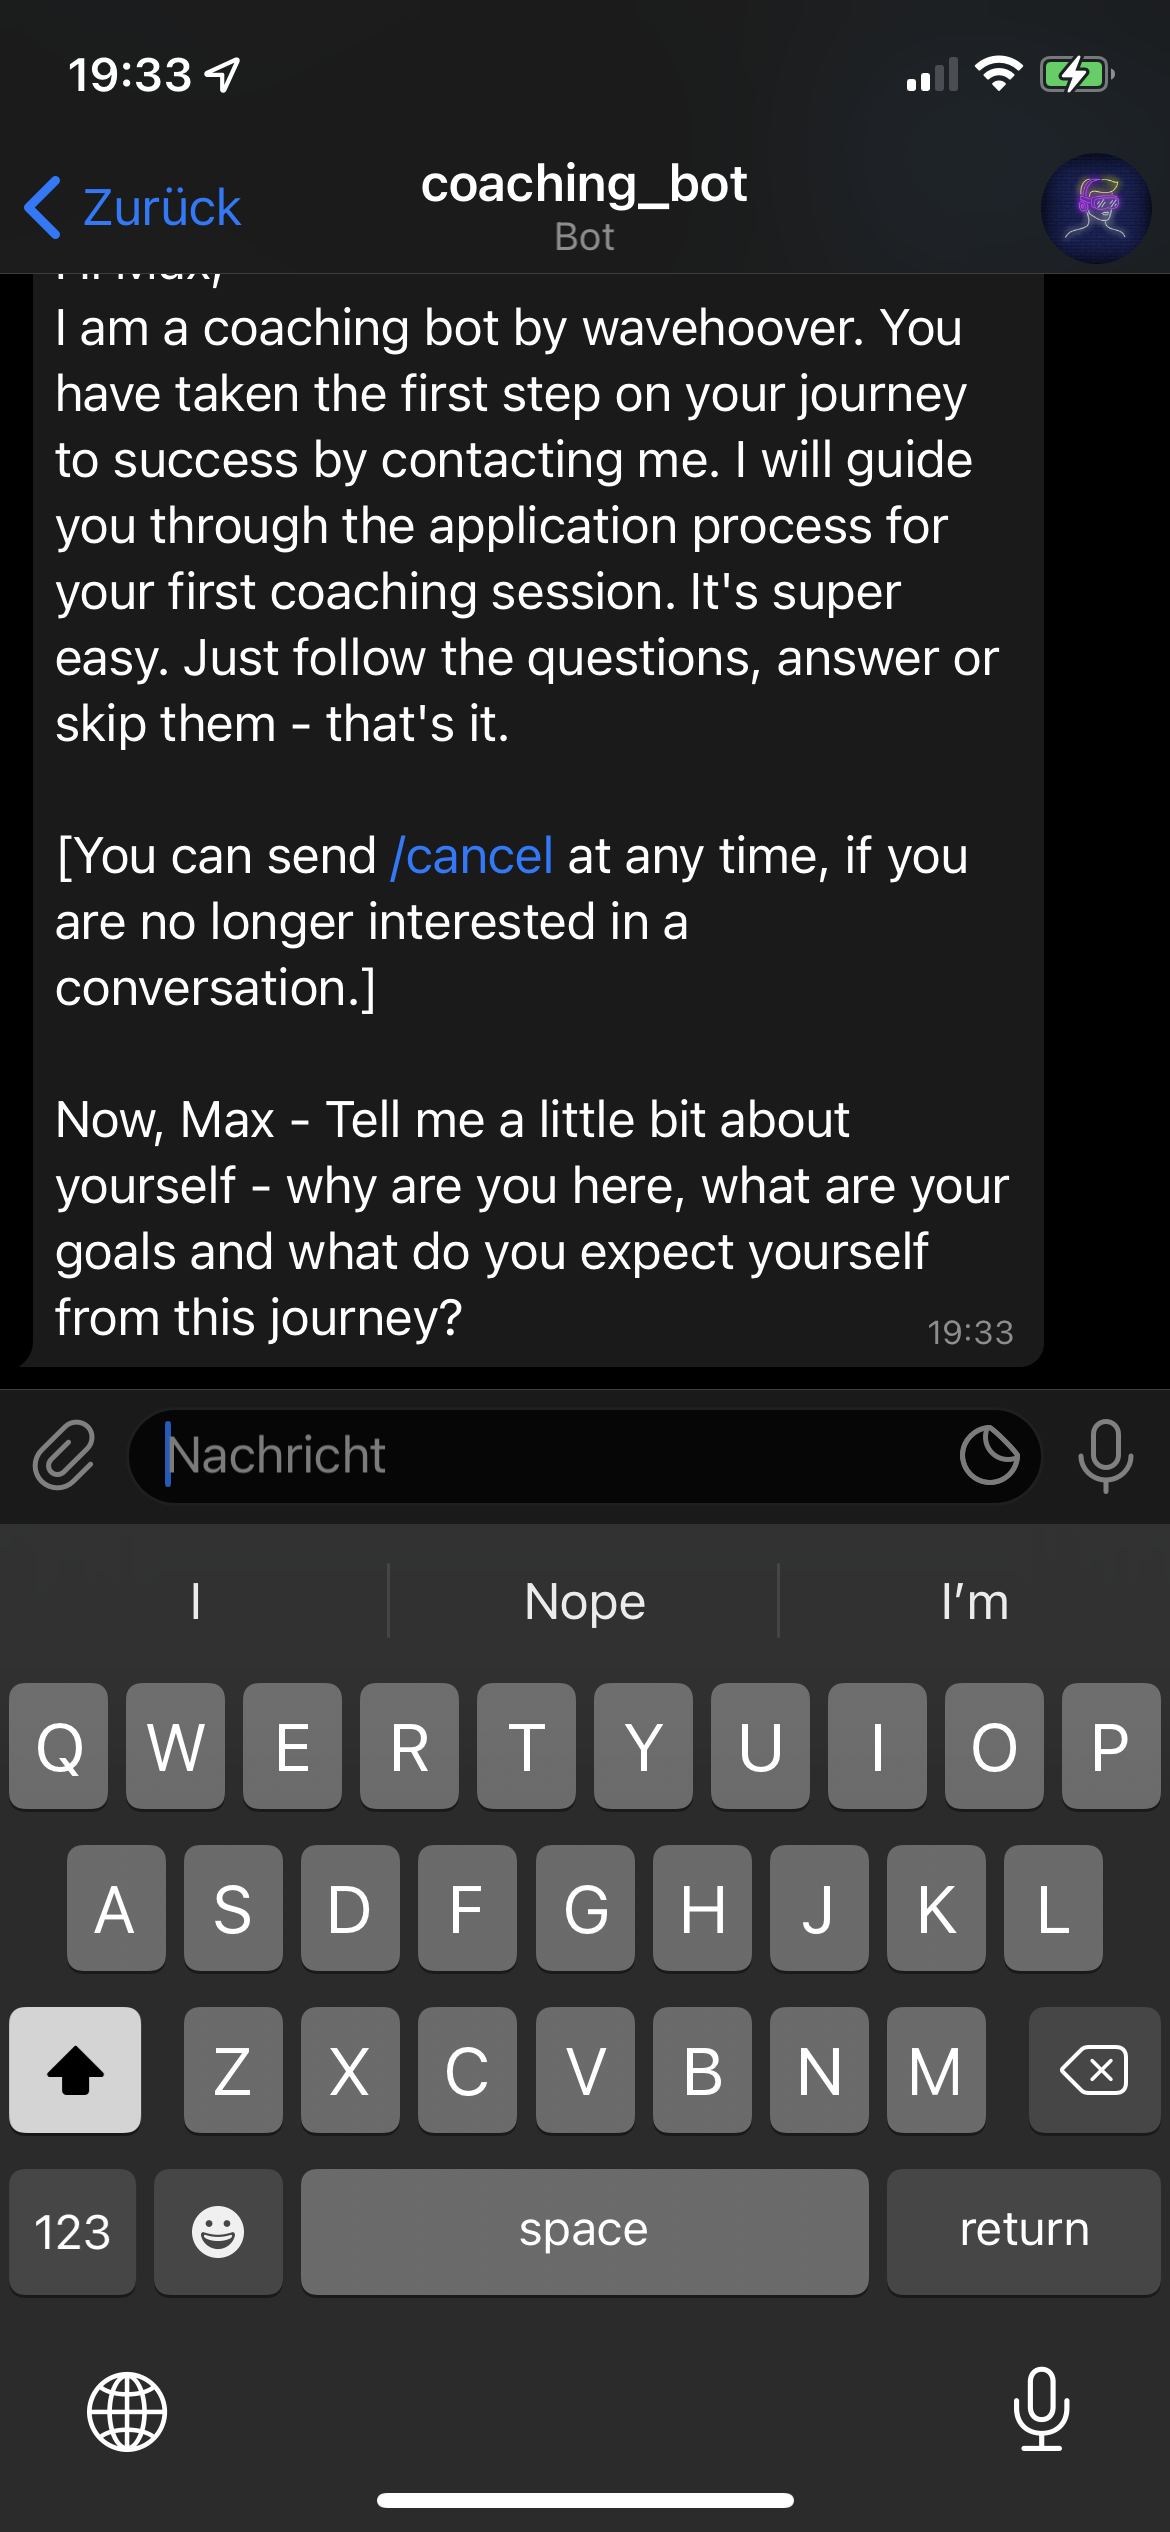
\includegraphics[width=\textwidth]{images/Screenshots/bio.PNG}
			\caption{Übergang zur Angabe der Biographie}
			\label{fig: scs..bio}
		\end{subfigure}

		\hfill
		
		\begin{subfigure}{0.3\textwidth}
			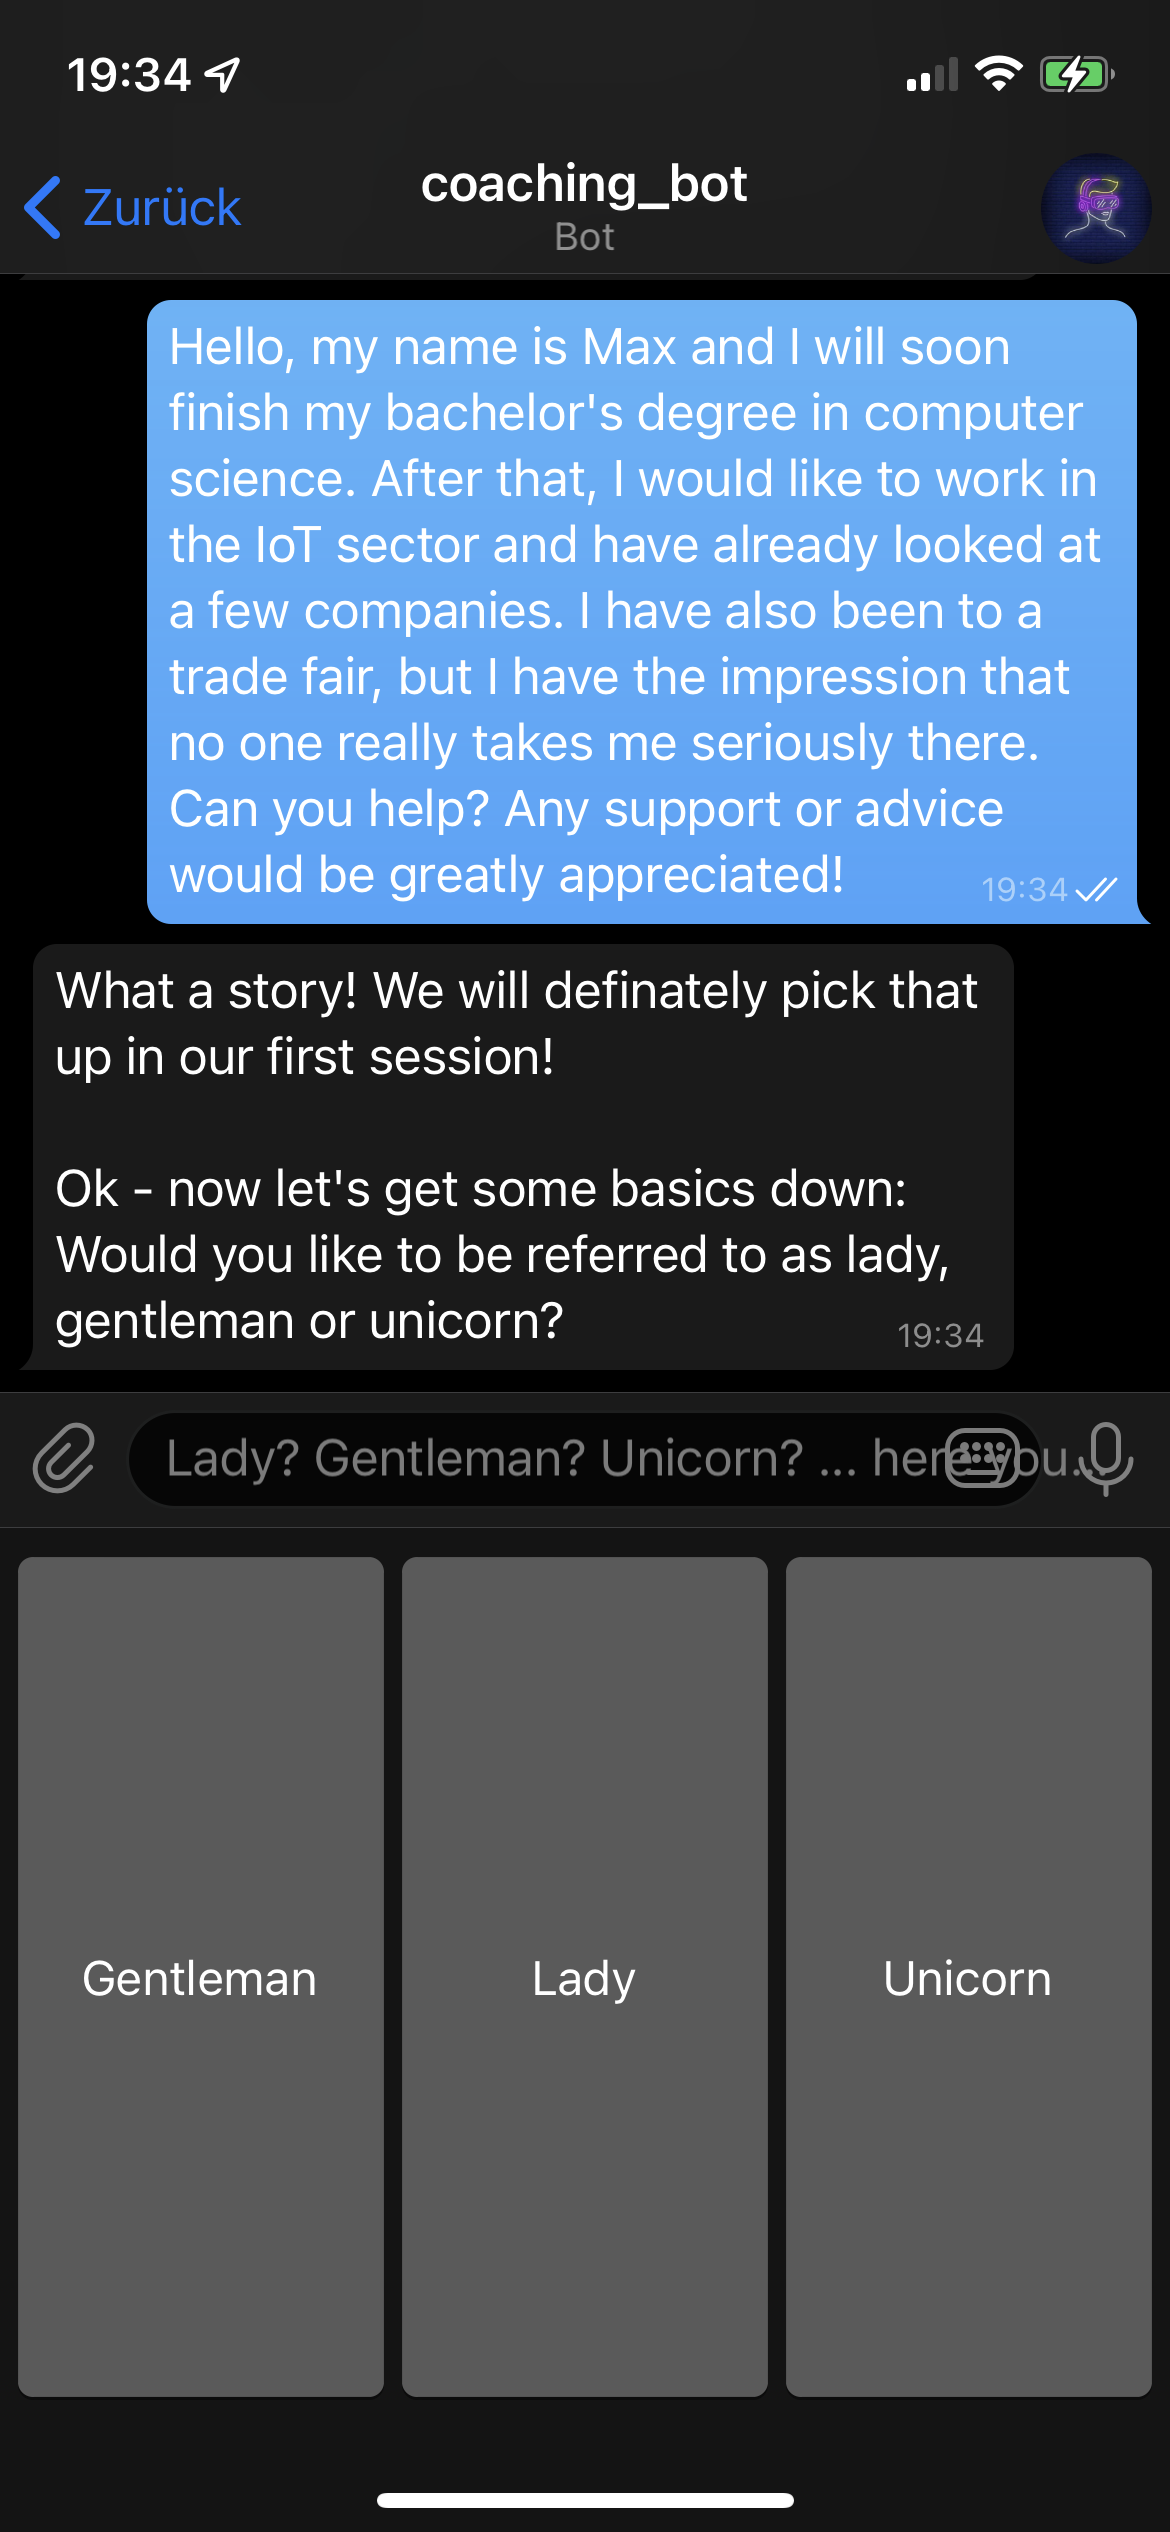
\includegraphics[width=\textwidth]{images/Screenshots/gender.PNG}
			\caption{Übergang zur Auswahl des Geschlechts}
			\label{fig: scs..gender}
		\end{subfigure}
				
		\caption{Creating subfigures in \LaTeX.}
		
		\label{fig:figures}

	\end{figure}

	% \begin{figure}[ht!]
	% 	\begin{center}

	% 		\subfigure[Einstieg via URL]{
	% 			\label{fig: scs..link}
	% 			
\includegraphics[width=0.4\textwidth]{images/Screenshots/link.png}
	% 		}
	% 		\subfigure[Start des CoachingBots]{
	% 			\label{fig: scs..start}
	% 			
\includegraphics[width=0.4\textwidth]{images/Screenshots/start.PNG}
	% 		}
	% 		\subfigure[Übergang zur Angabe der Biographie]{
	% 			\label{fig: scs..bio}
	% 			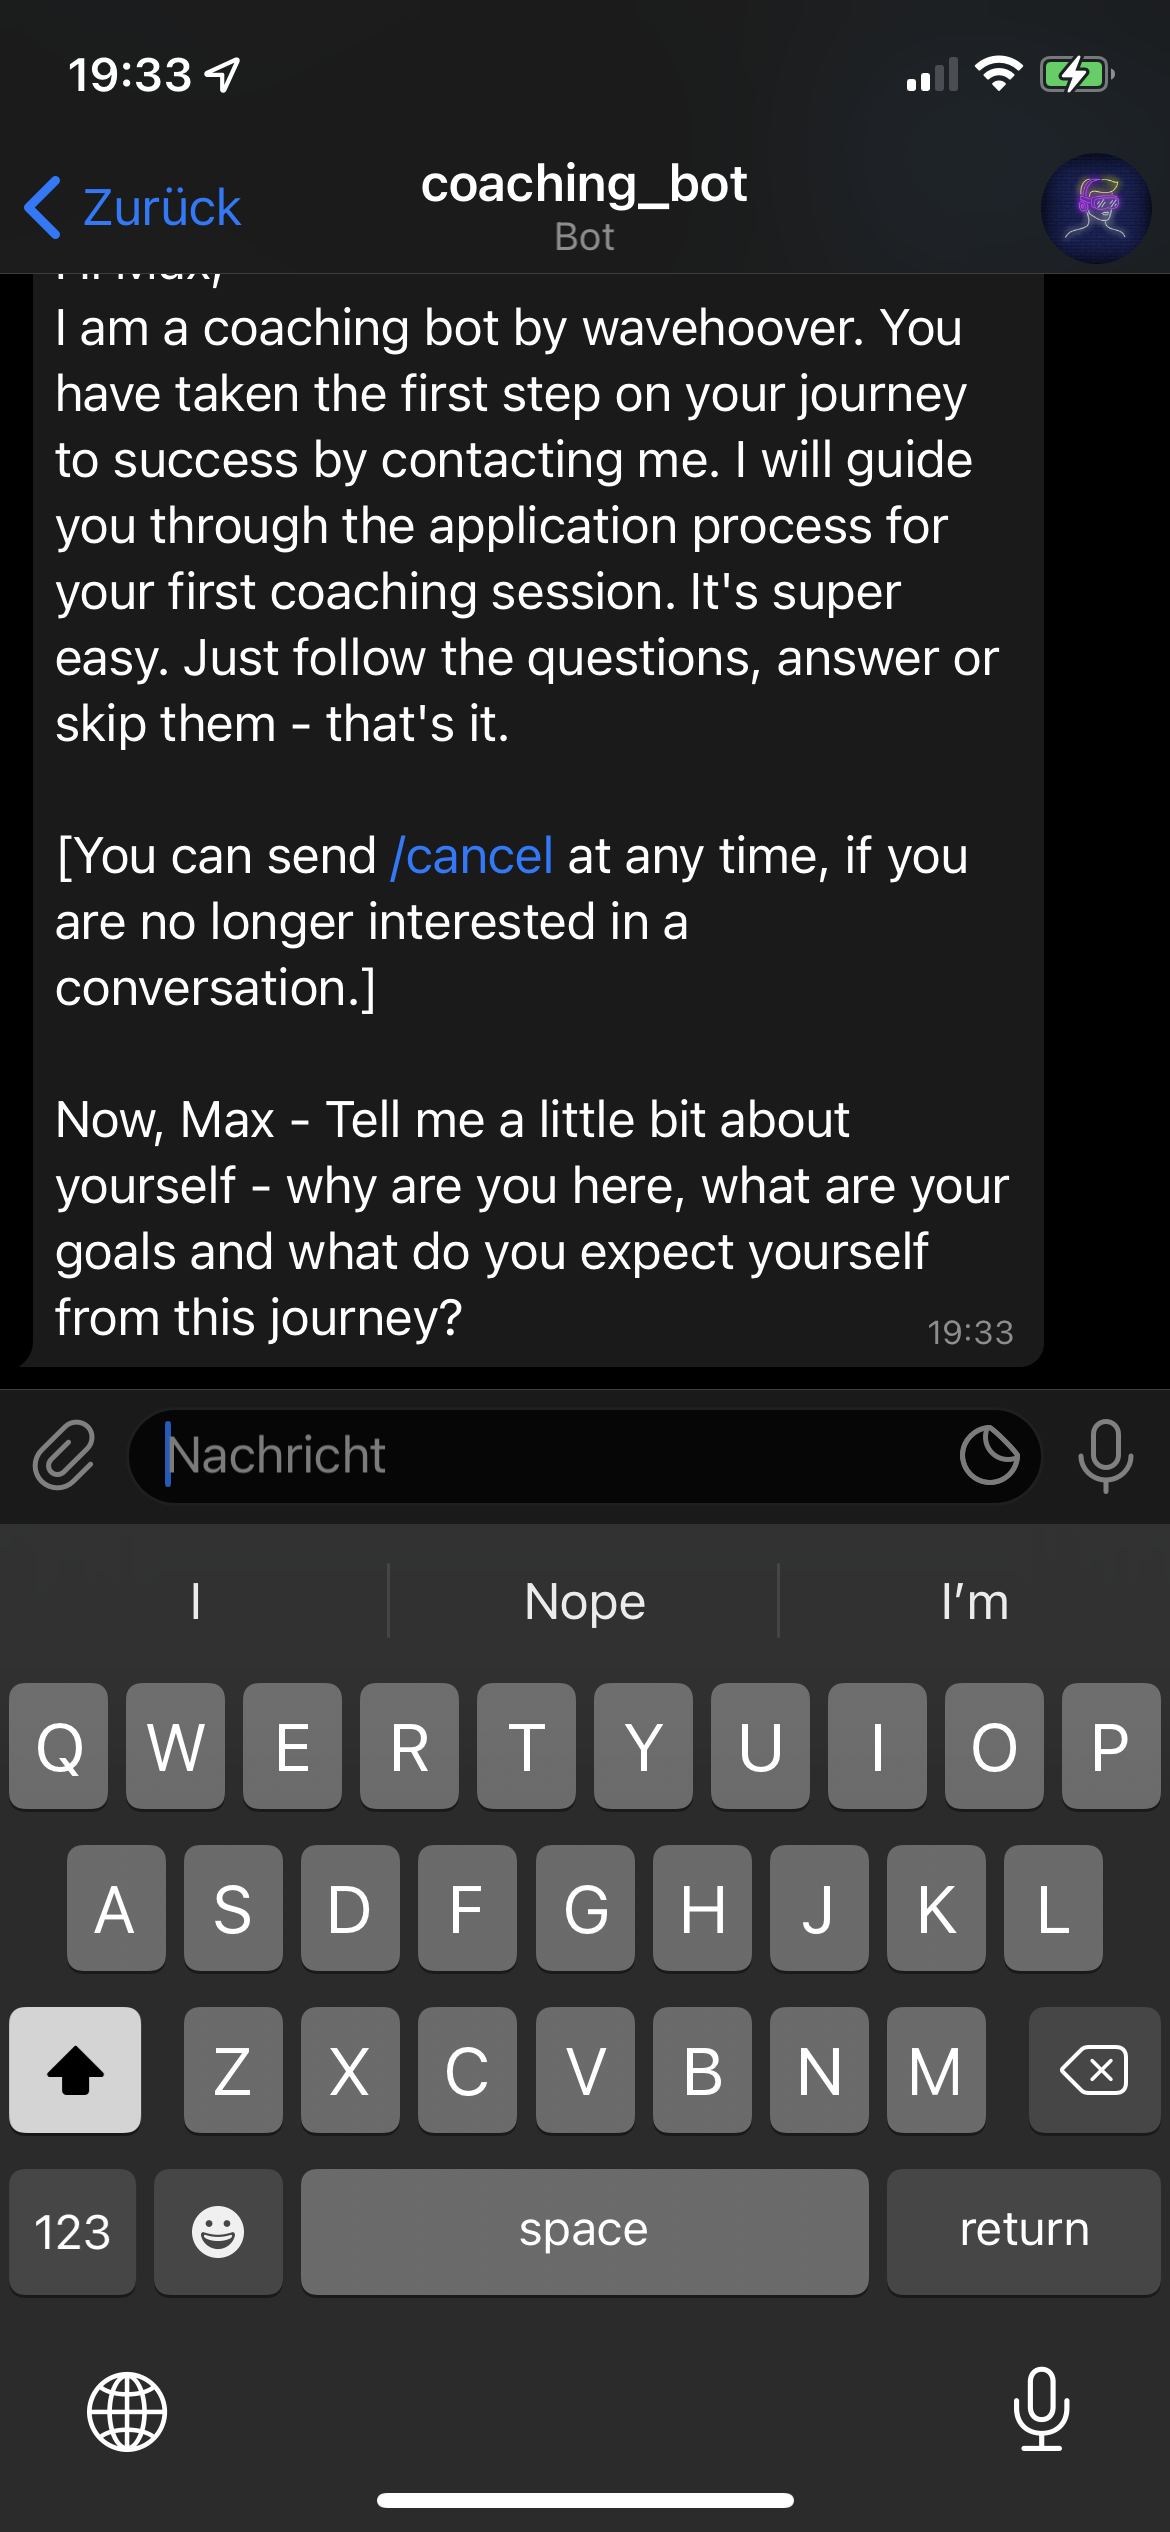
\includegraphics[width=0.4\textwidth]{images/Screenshots/bio.PNG}
	% 		}
	% 		\subfigure[Übergang zur Auswahl des Geschlechts]{
	% 			\label{fig: scs..gender}
	% 			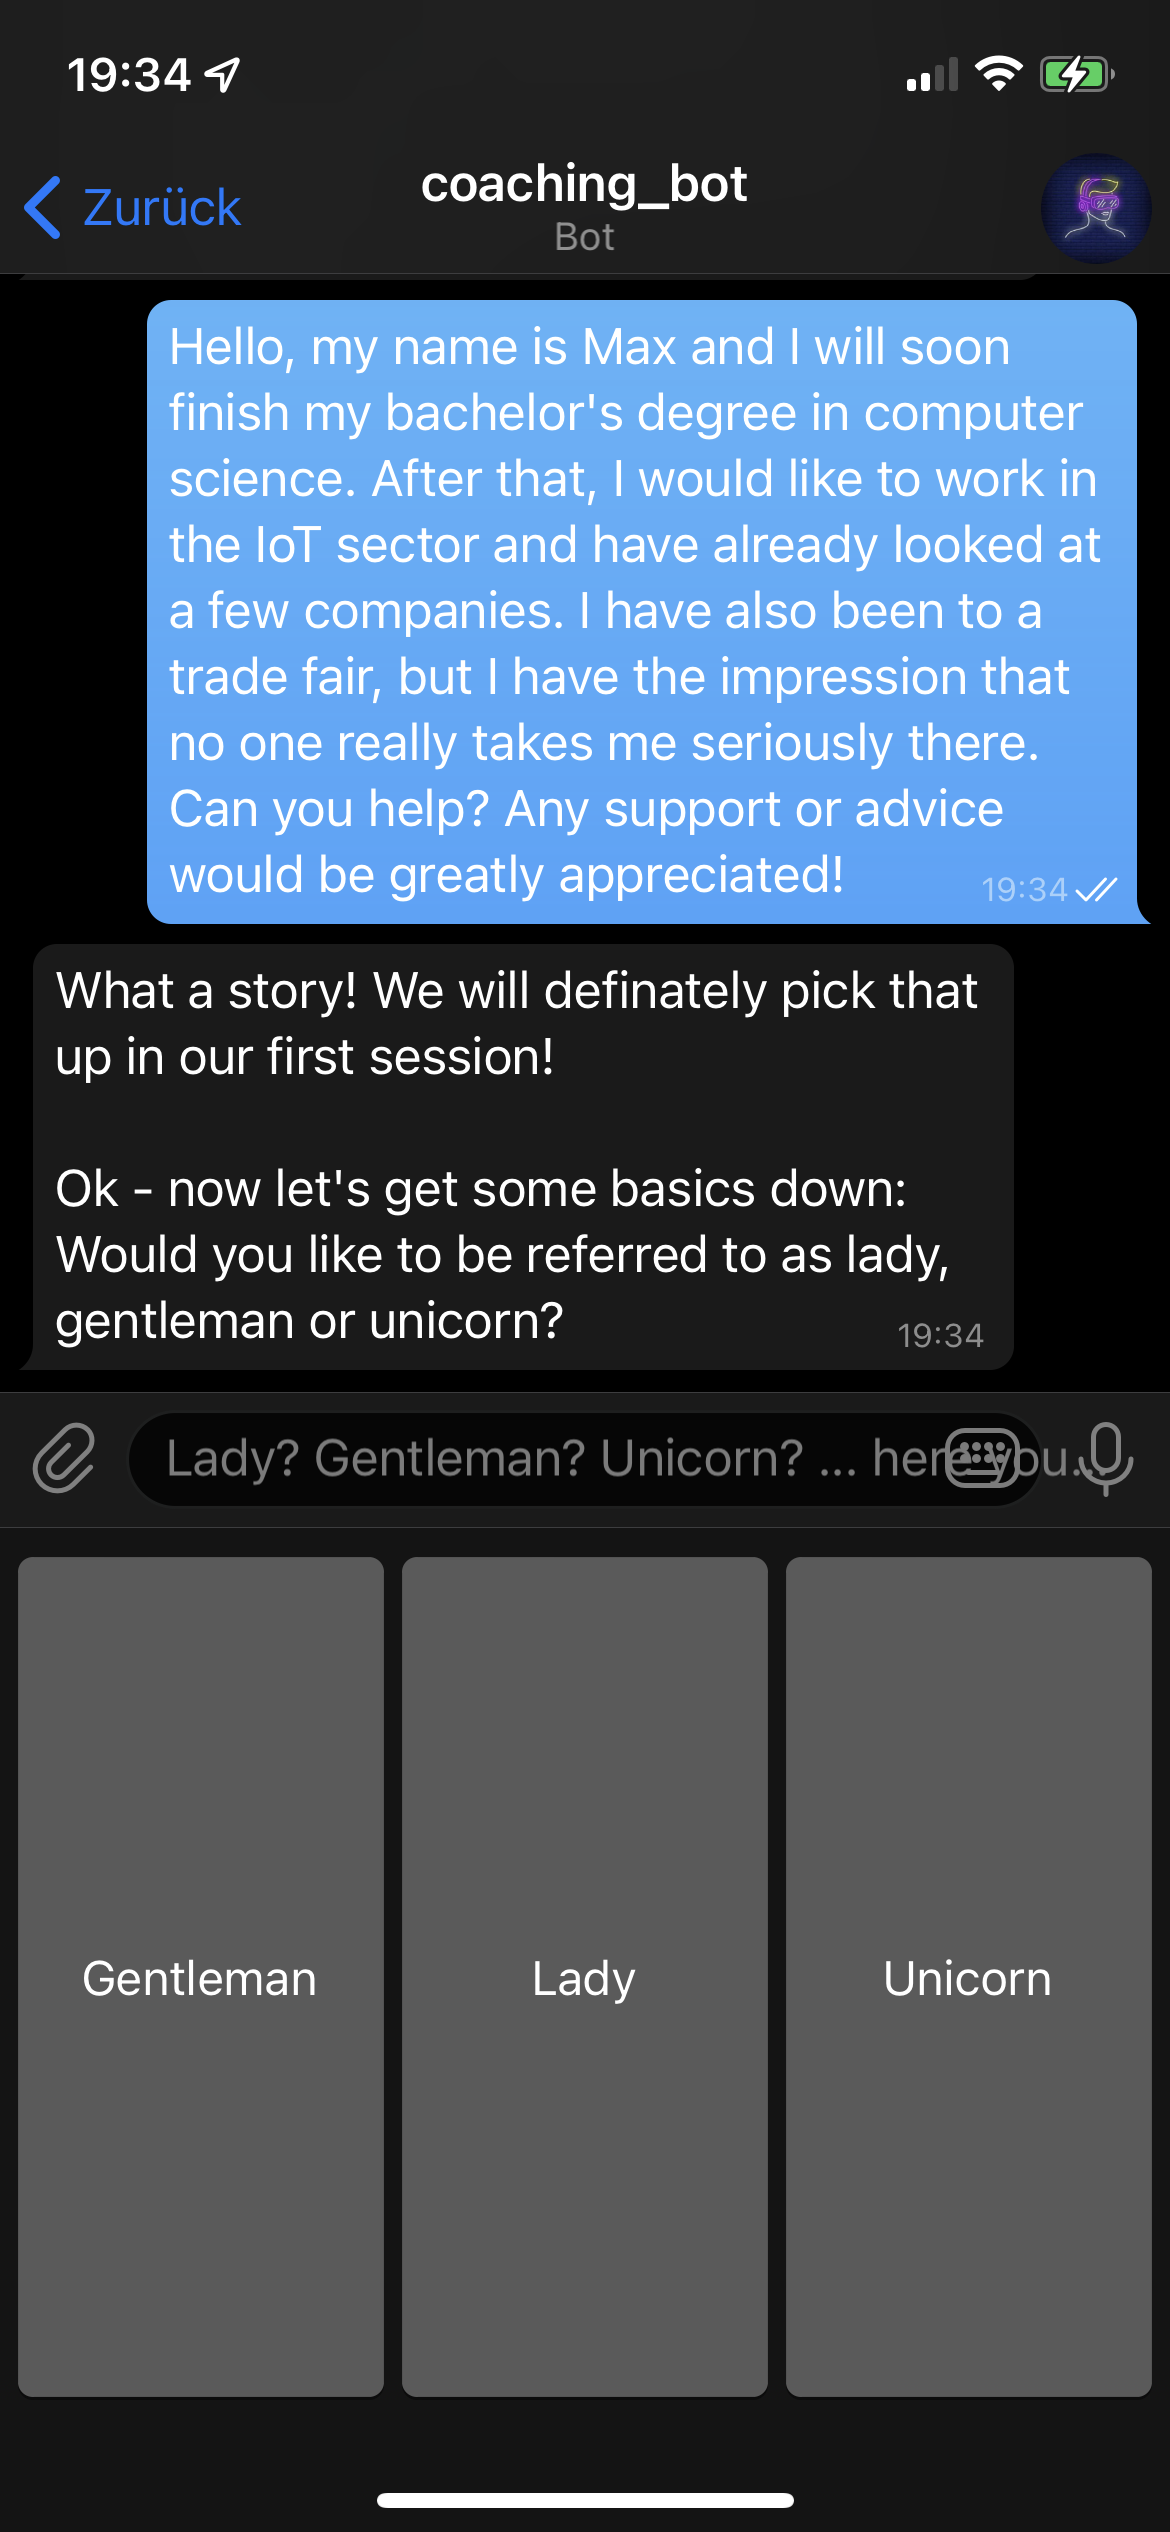
\includegraphics[width=0.4\textwidth]{images/Screenshots/gender.PNG}
	% 		}
	% 	\end{center}
	% 	\caption{
    %     Der Nutzer kommt im Bot an und er sieht einen Start-Button. Wenn er diesen drückt, wird die erste Nachricht an den Nutzer ausgegeben. Nun beginnt der Kommunikationsfluss zwischen Nutzer und Bot. Hier zusehen die ersten zwei Zustände und die Übergänge zu ihnen. (BIO und GENDER)
    %  	}
	% 	\label{fig: scs..page1 - start}
	% \end{figure}


	\begin{figure}
		\centering
		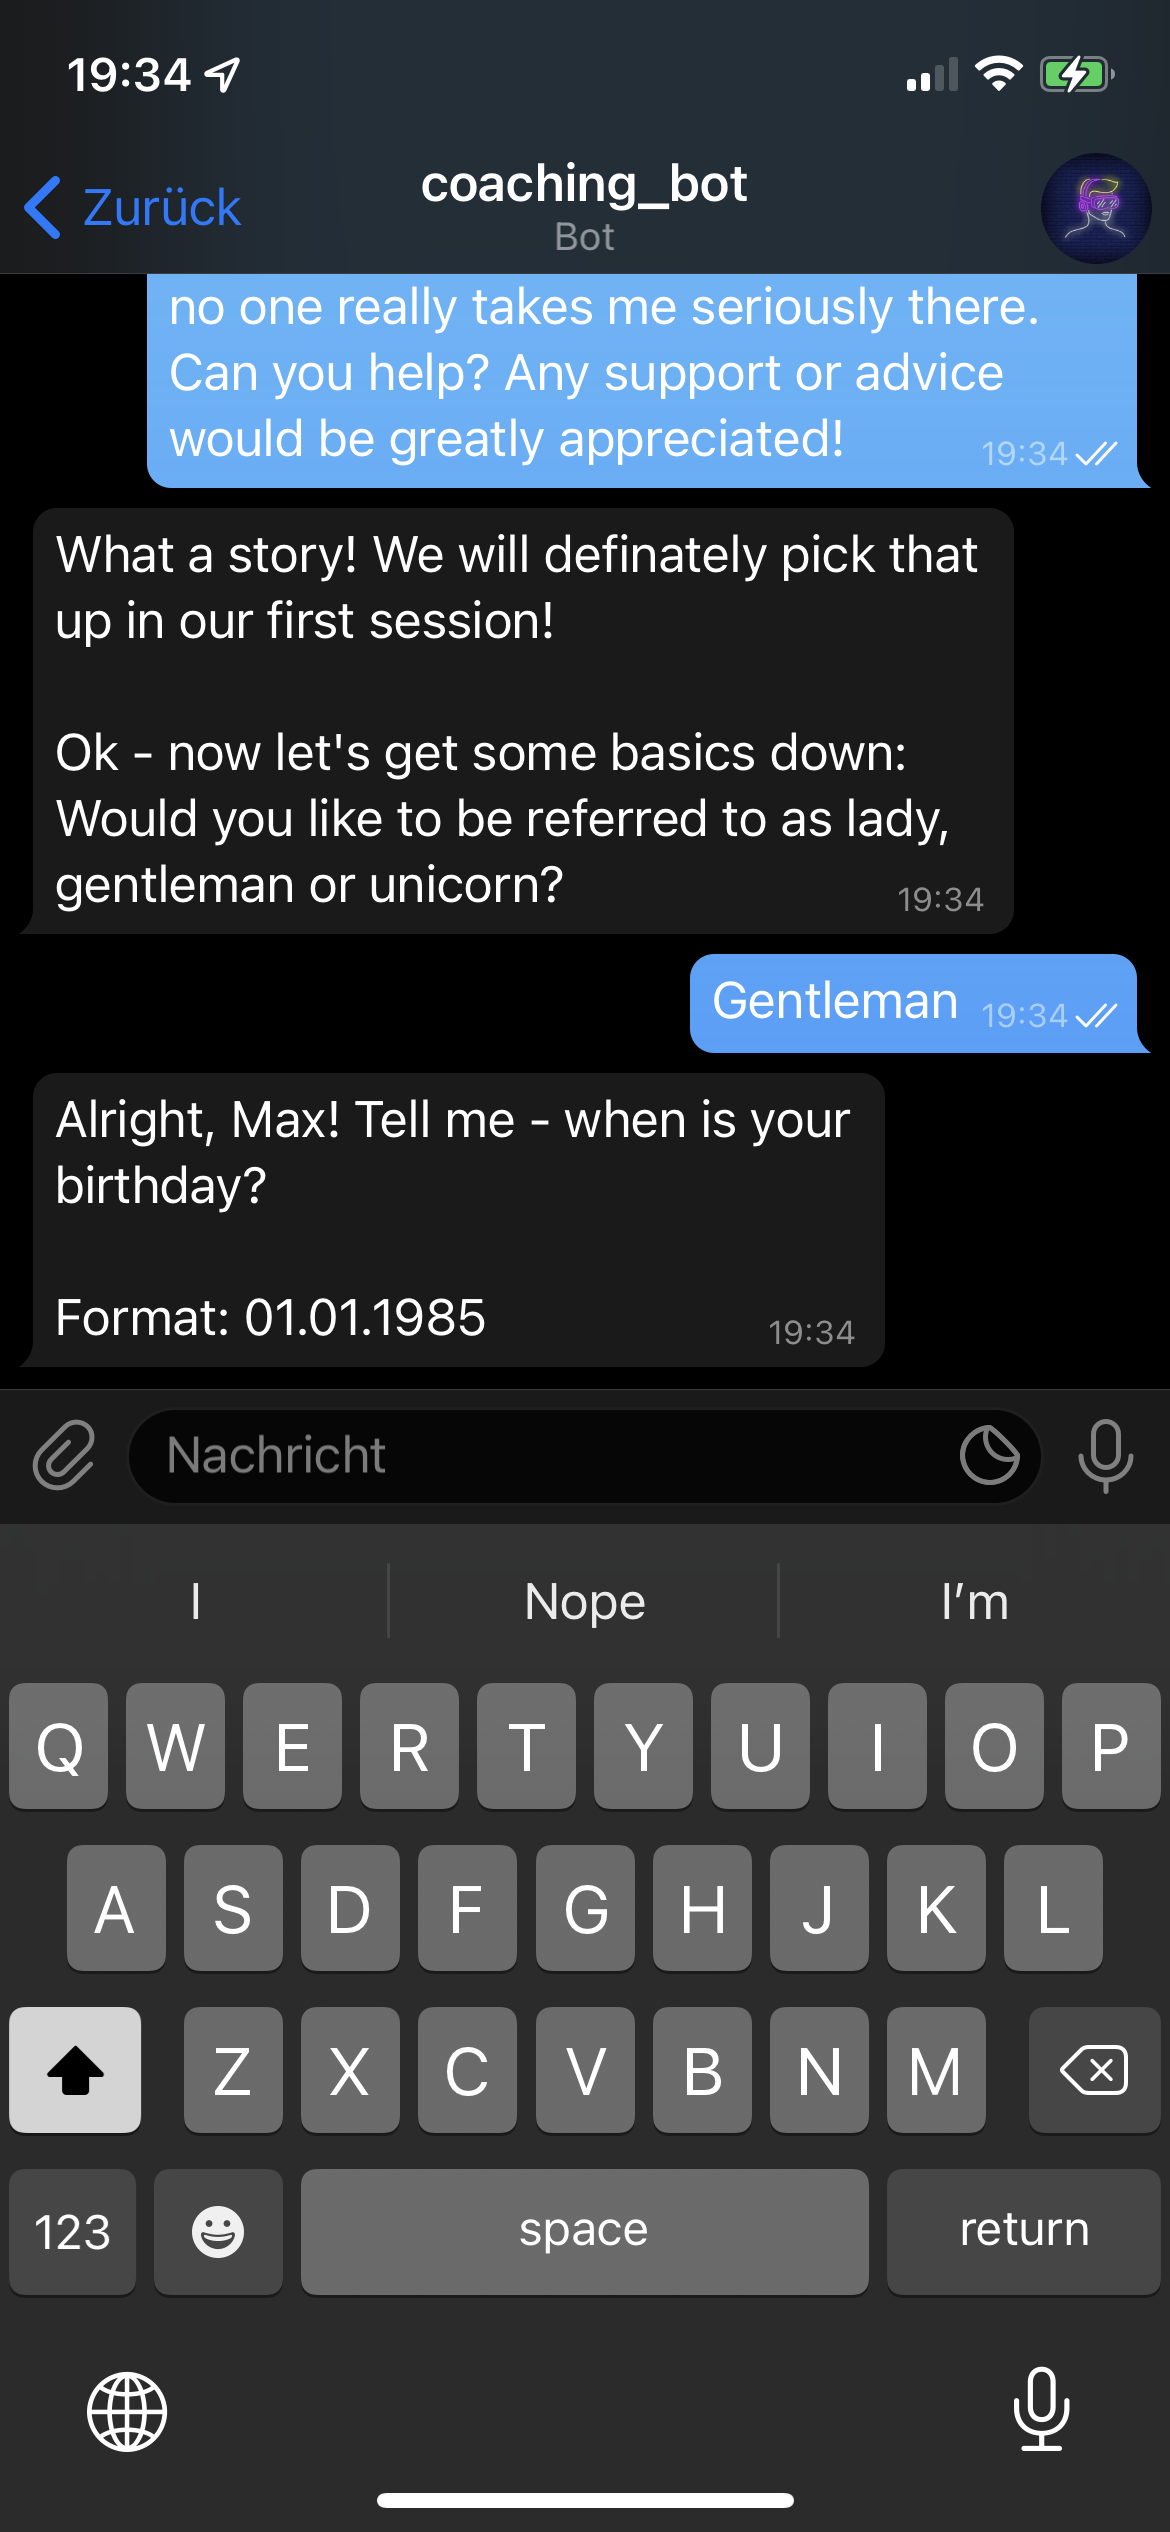
\includegraphics[width=0.4\textwidth]{images/Screenshots/birthdate.PNG}
		\caption{Übergang zur Angabe des Geburtsdatums}
		\label{fig: scs..birthdate}
	\end{figure}


	\begin{figure}
		\centering
		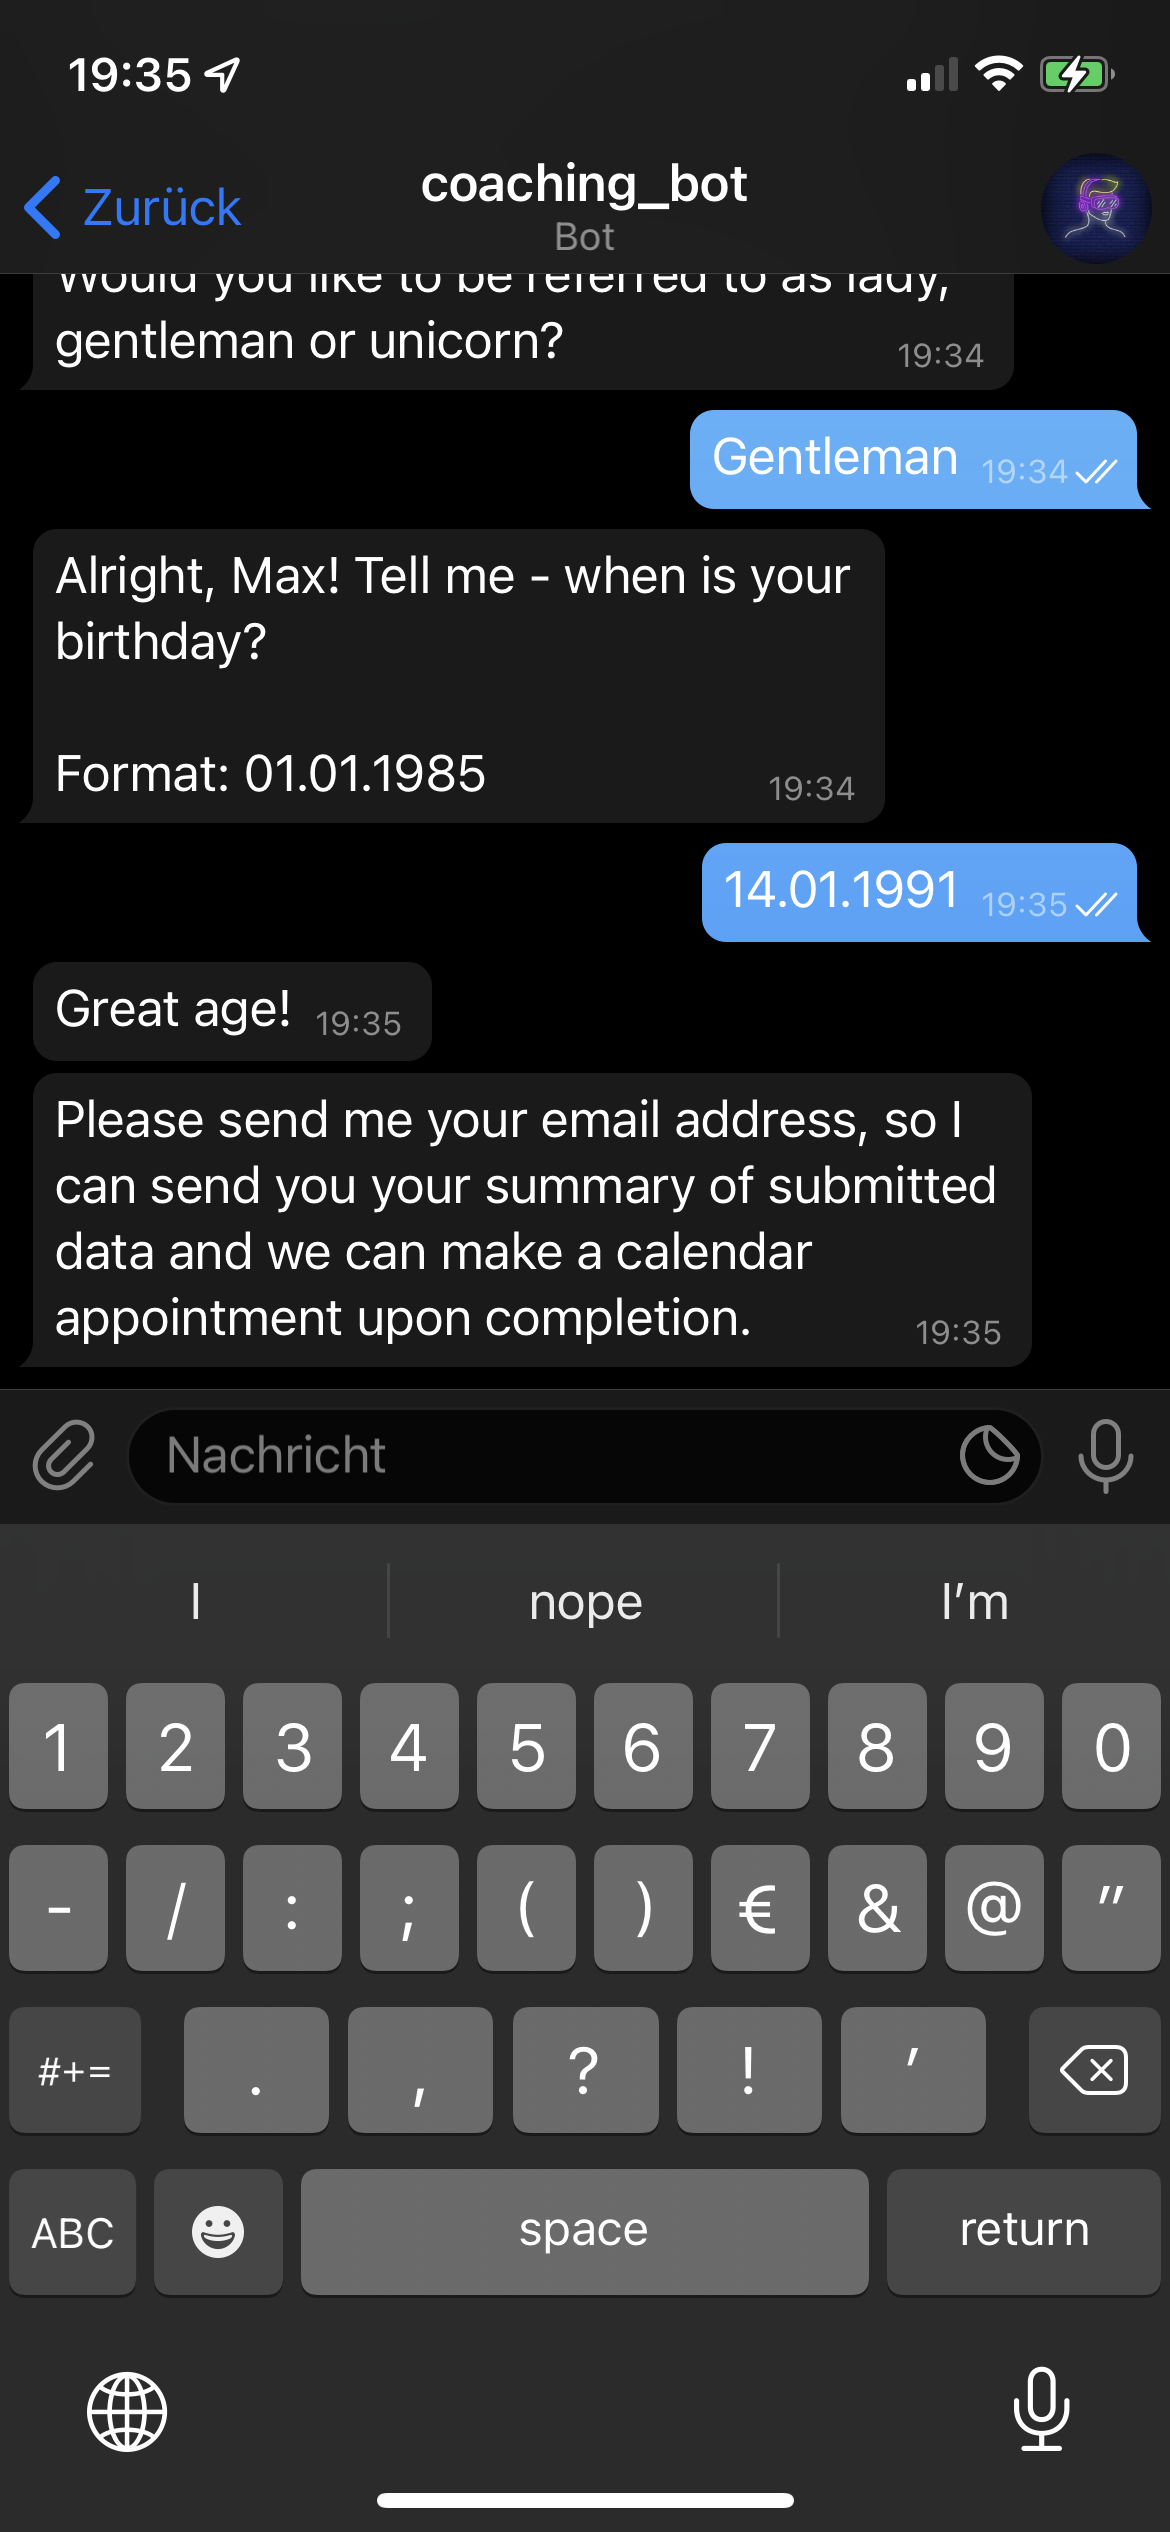
\includegraphics[width=0.4\textwidth]{images/Screenshots/email.PNG}
		\caption{Übergang zur Angabe der E-Mail-Adresse}
		\label{fig: scs..email}
	\end{figure}


	\begin{figure}
		\centering
		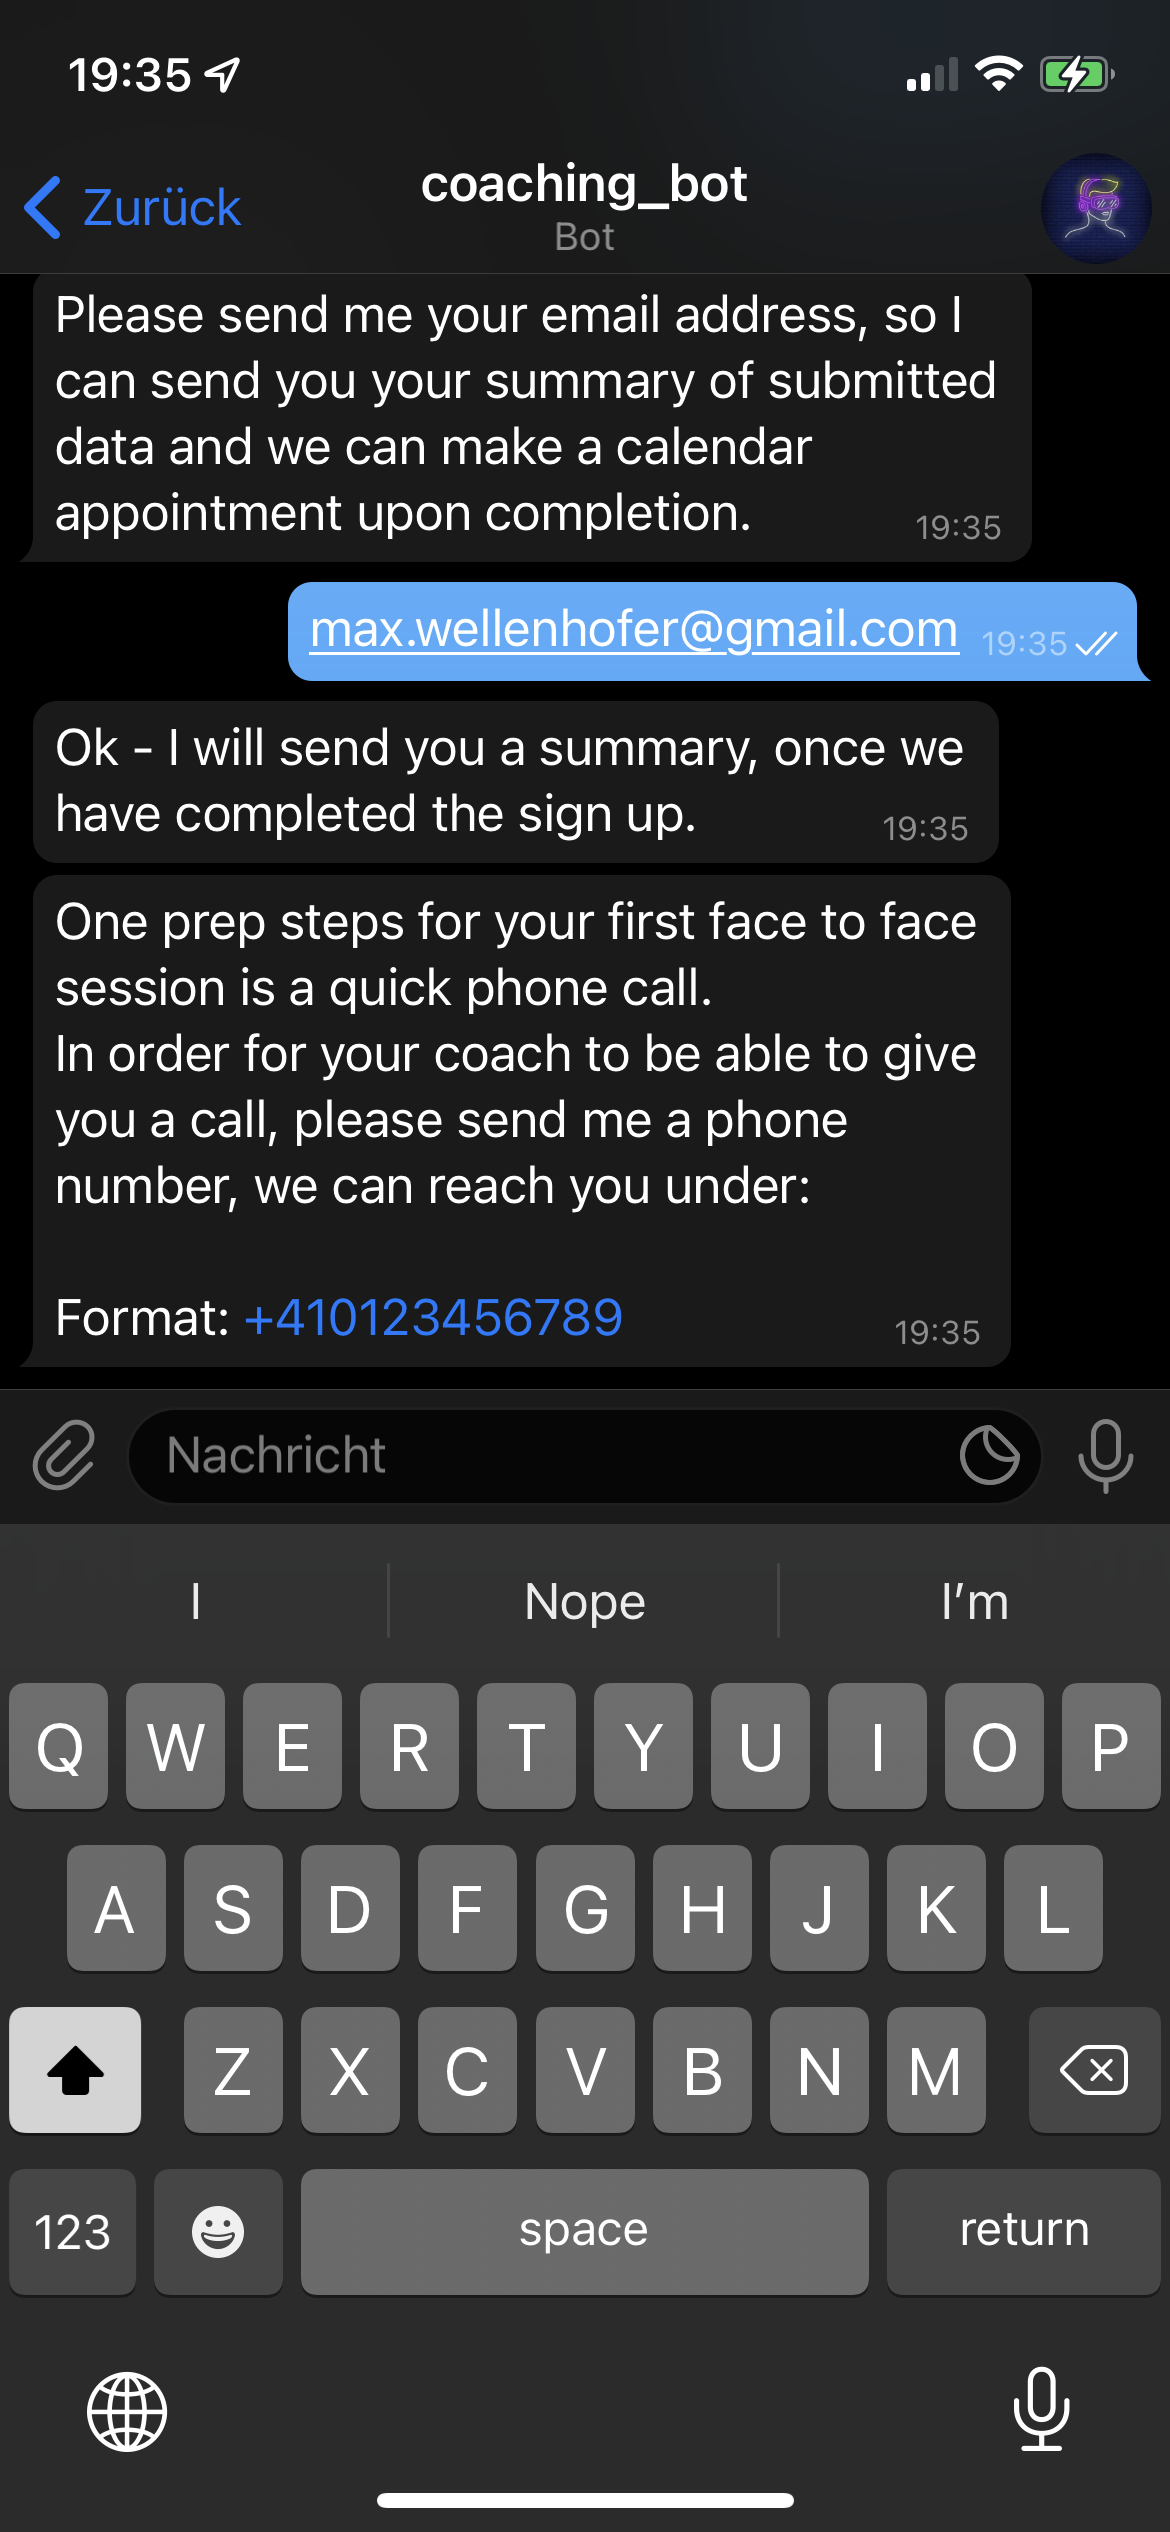
\includegraphics[width=0.4\textwidth]{images/Screenshots/telephone.PNG}
		\caption{Übergang zur Angabe der Telefonnummer}
		\label{fig: scs..telephone}
	\end{figure}


	\begin{figure}
		\centering
		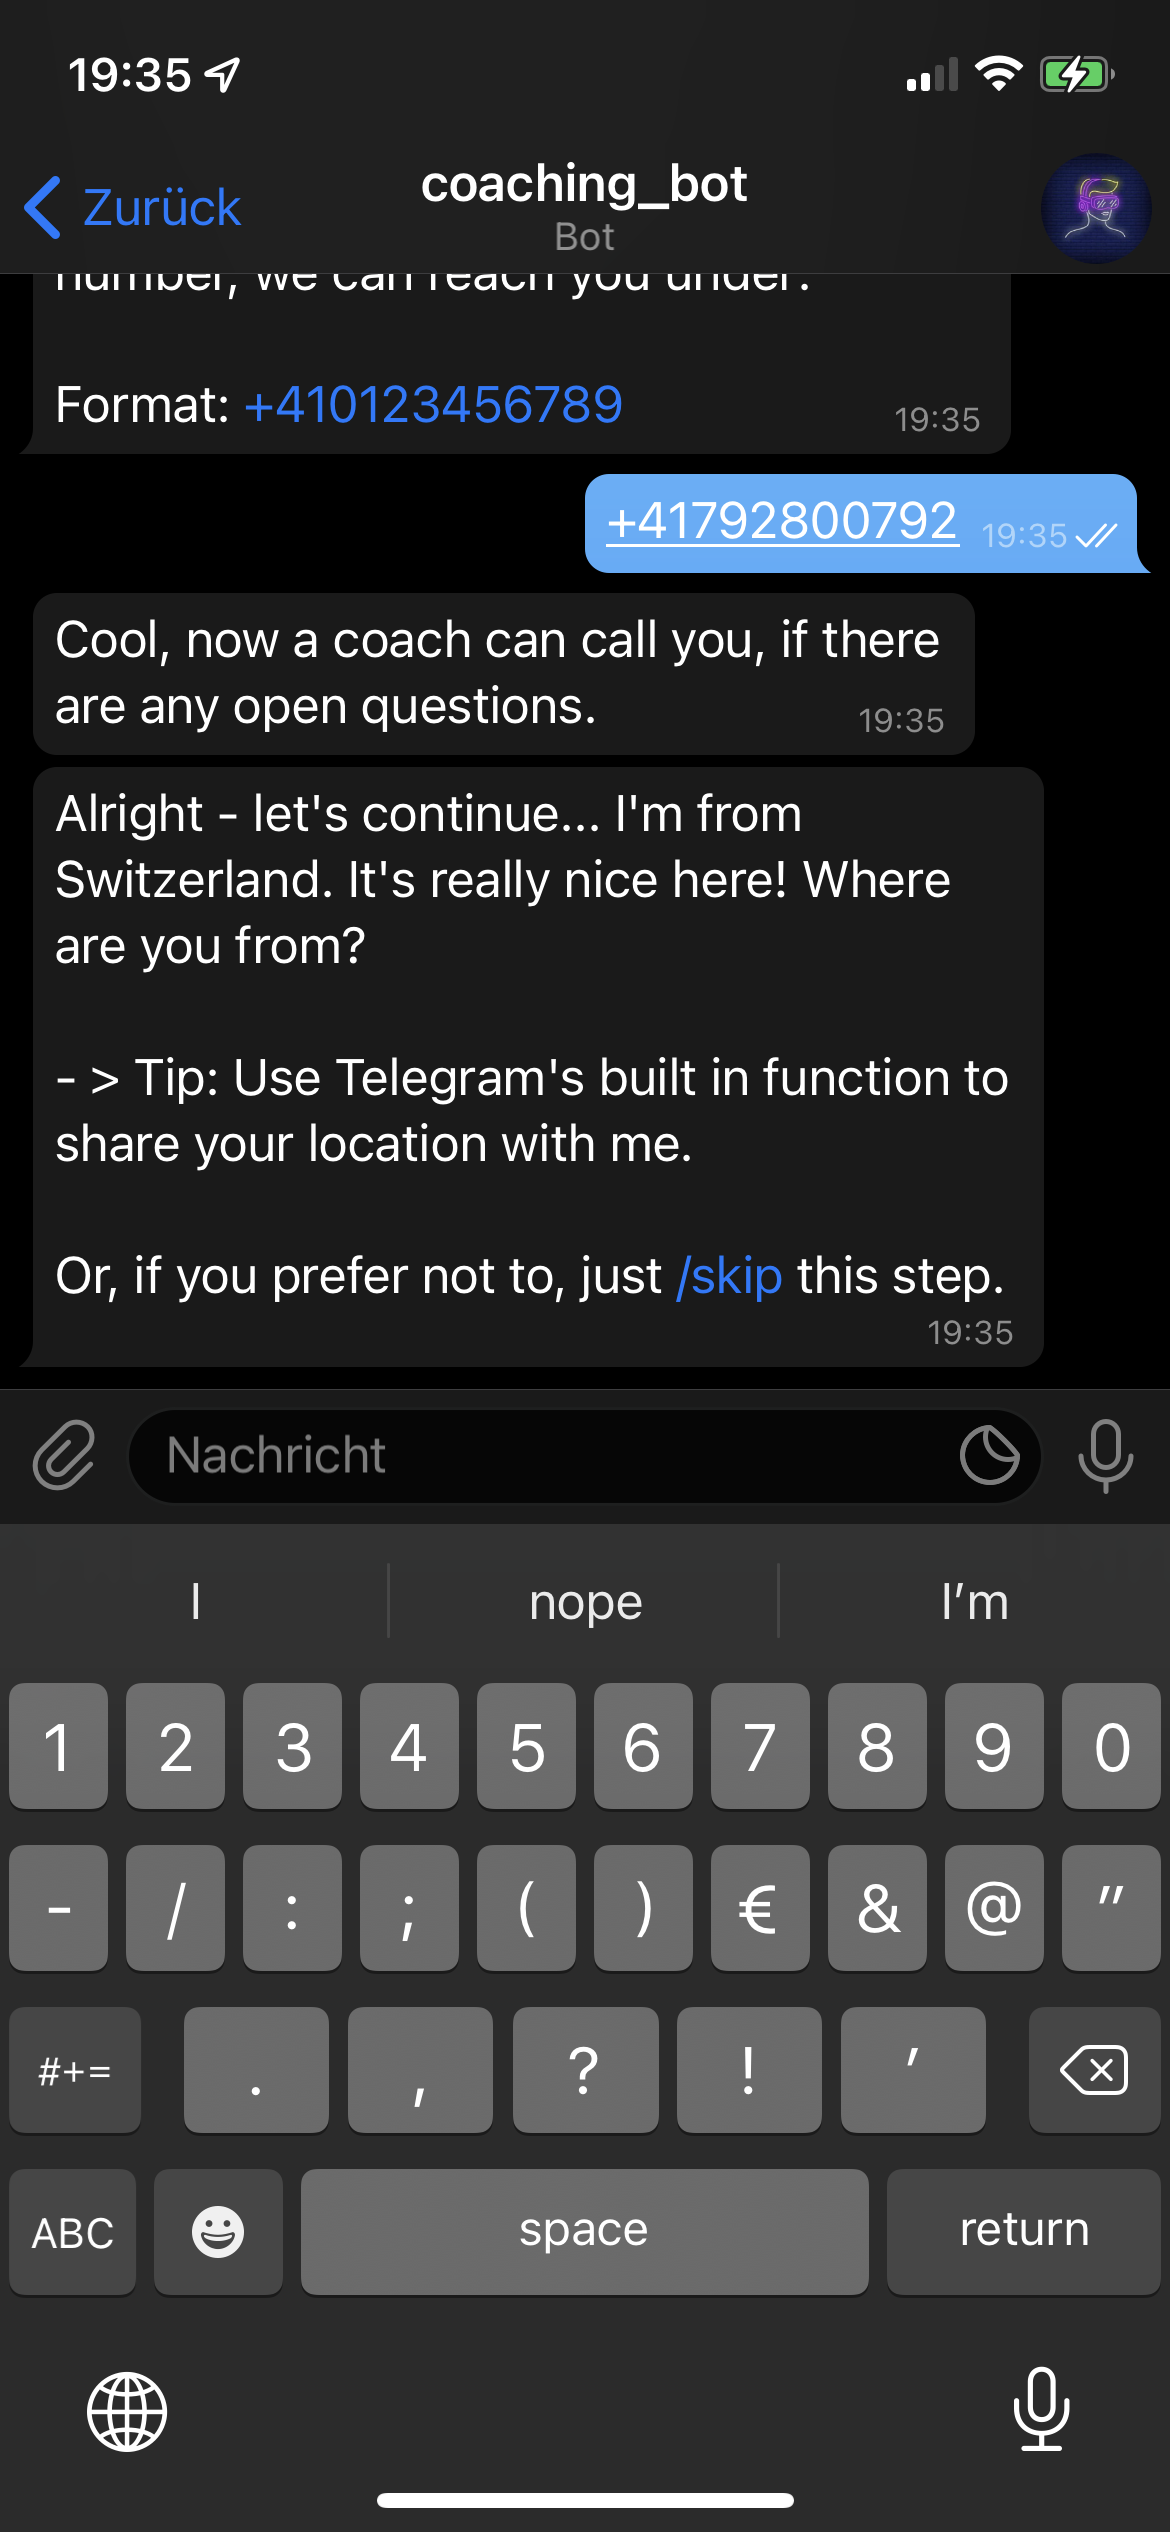
\includegraphics[width=0.4\textwidth]{images/Screenshots/location.PNG}
		\caption{Übergang zur Angabe des Standorts}
		\label{fig: scs..location}
	\end{figure}


	\begin{figure}
		\centering
		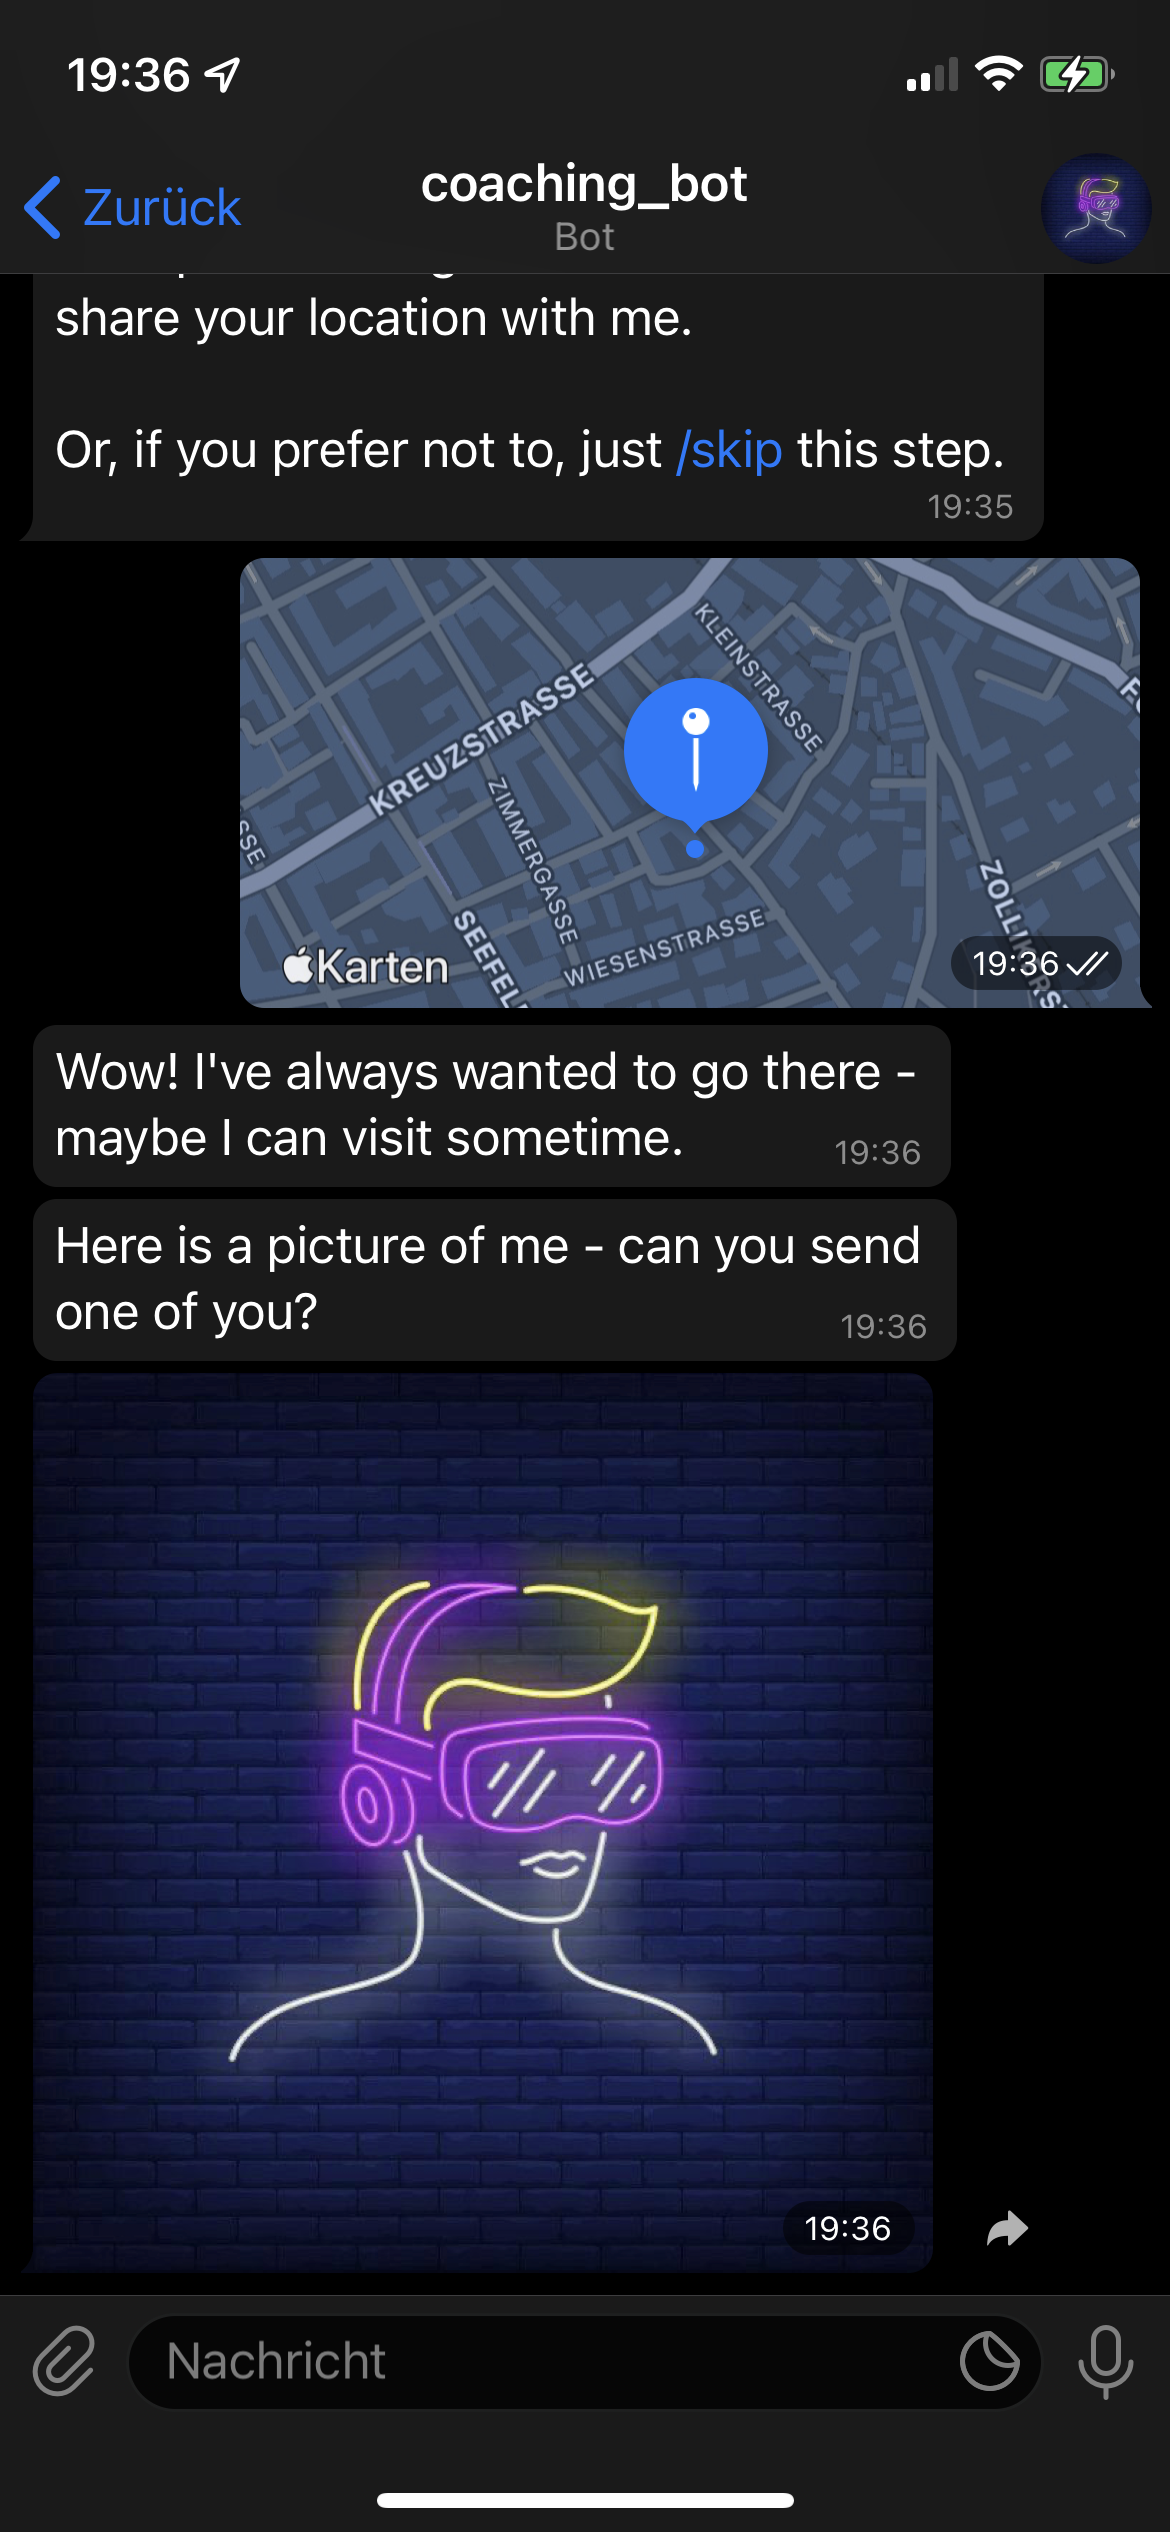
\includegraphics[width=0.4\textwidth]{images/Screenshots/photo.PNG}
		\caption{Übergang zum Upload eines Fotos}
		\label{fig: scs..photo}
	\end{figure}


	\begin{figure}
		\centering
		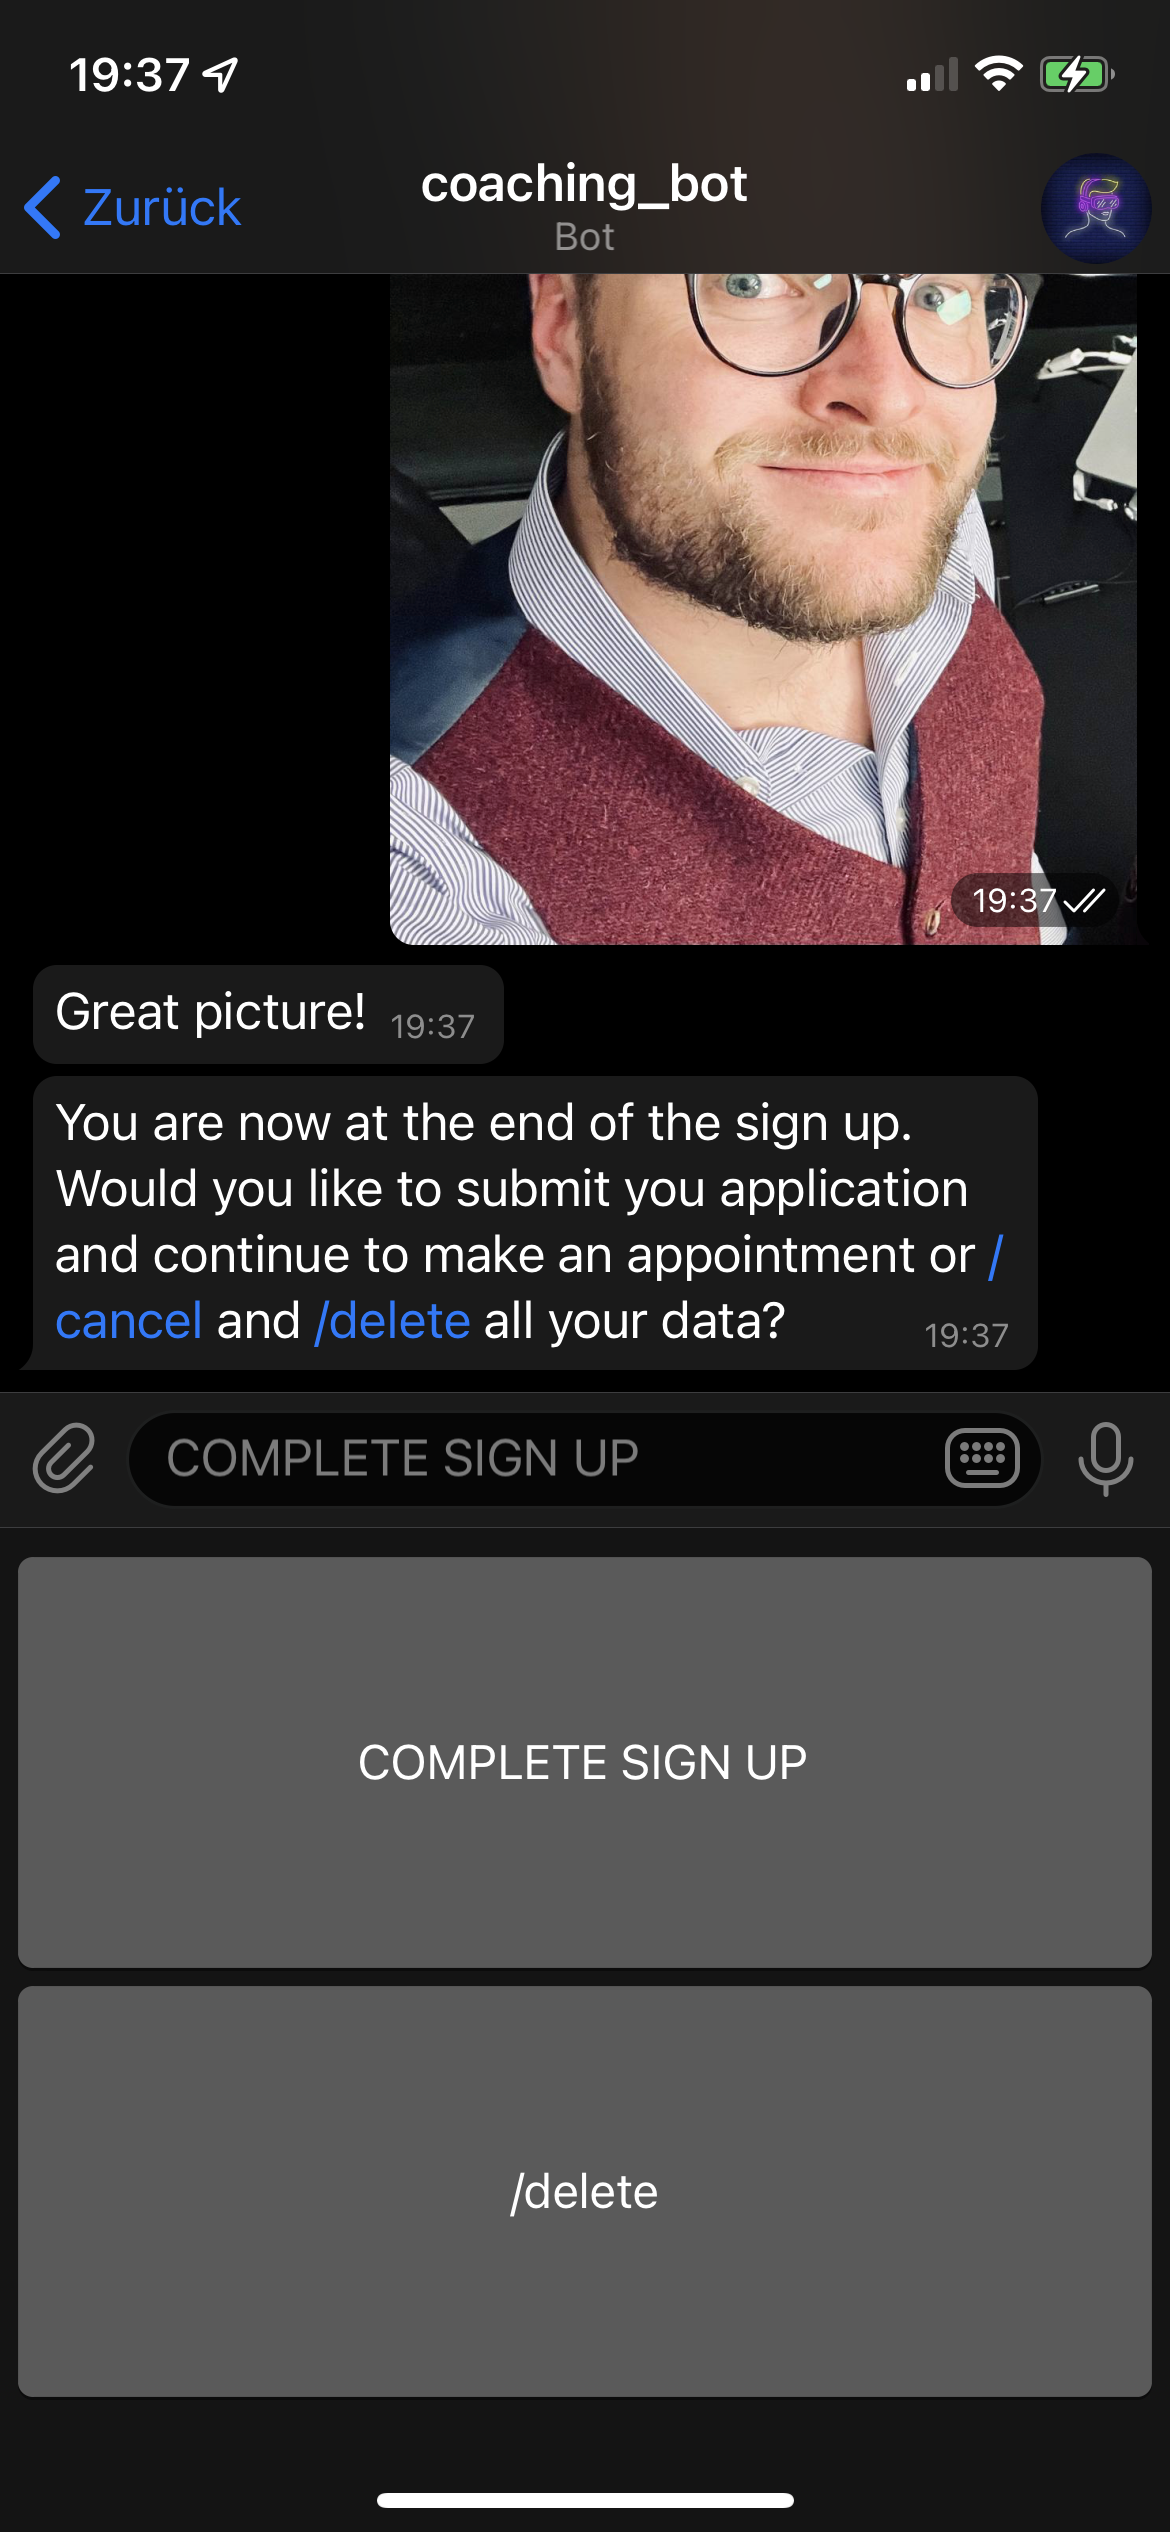
\includegraphics[width=0.4\textwidth]{images/Screenshots/complete-sign-up.PNG}
		\caption{Ende der Anmeldung und Übergang zur Terminauswahl}
		\label{fig: scs..complete-sign-up}
	\end{figure}


	\begin{figure}
		\centering
		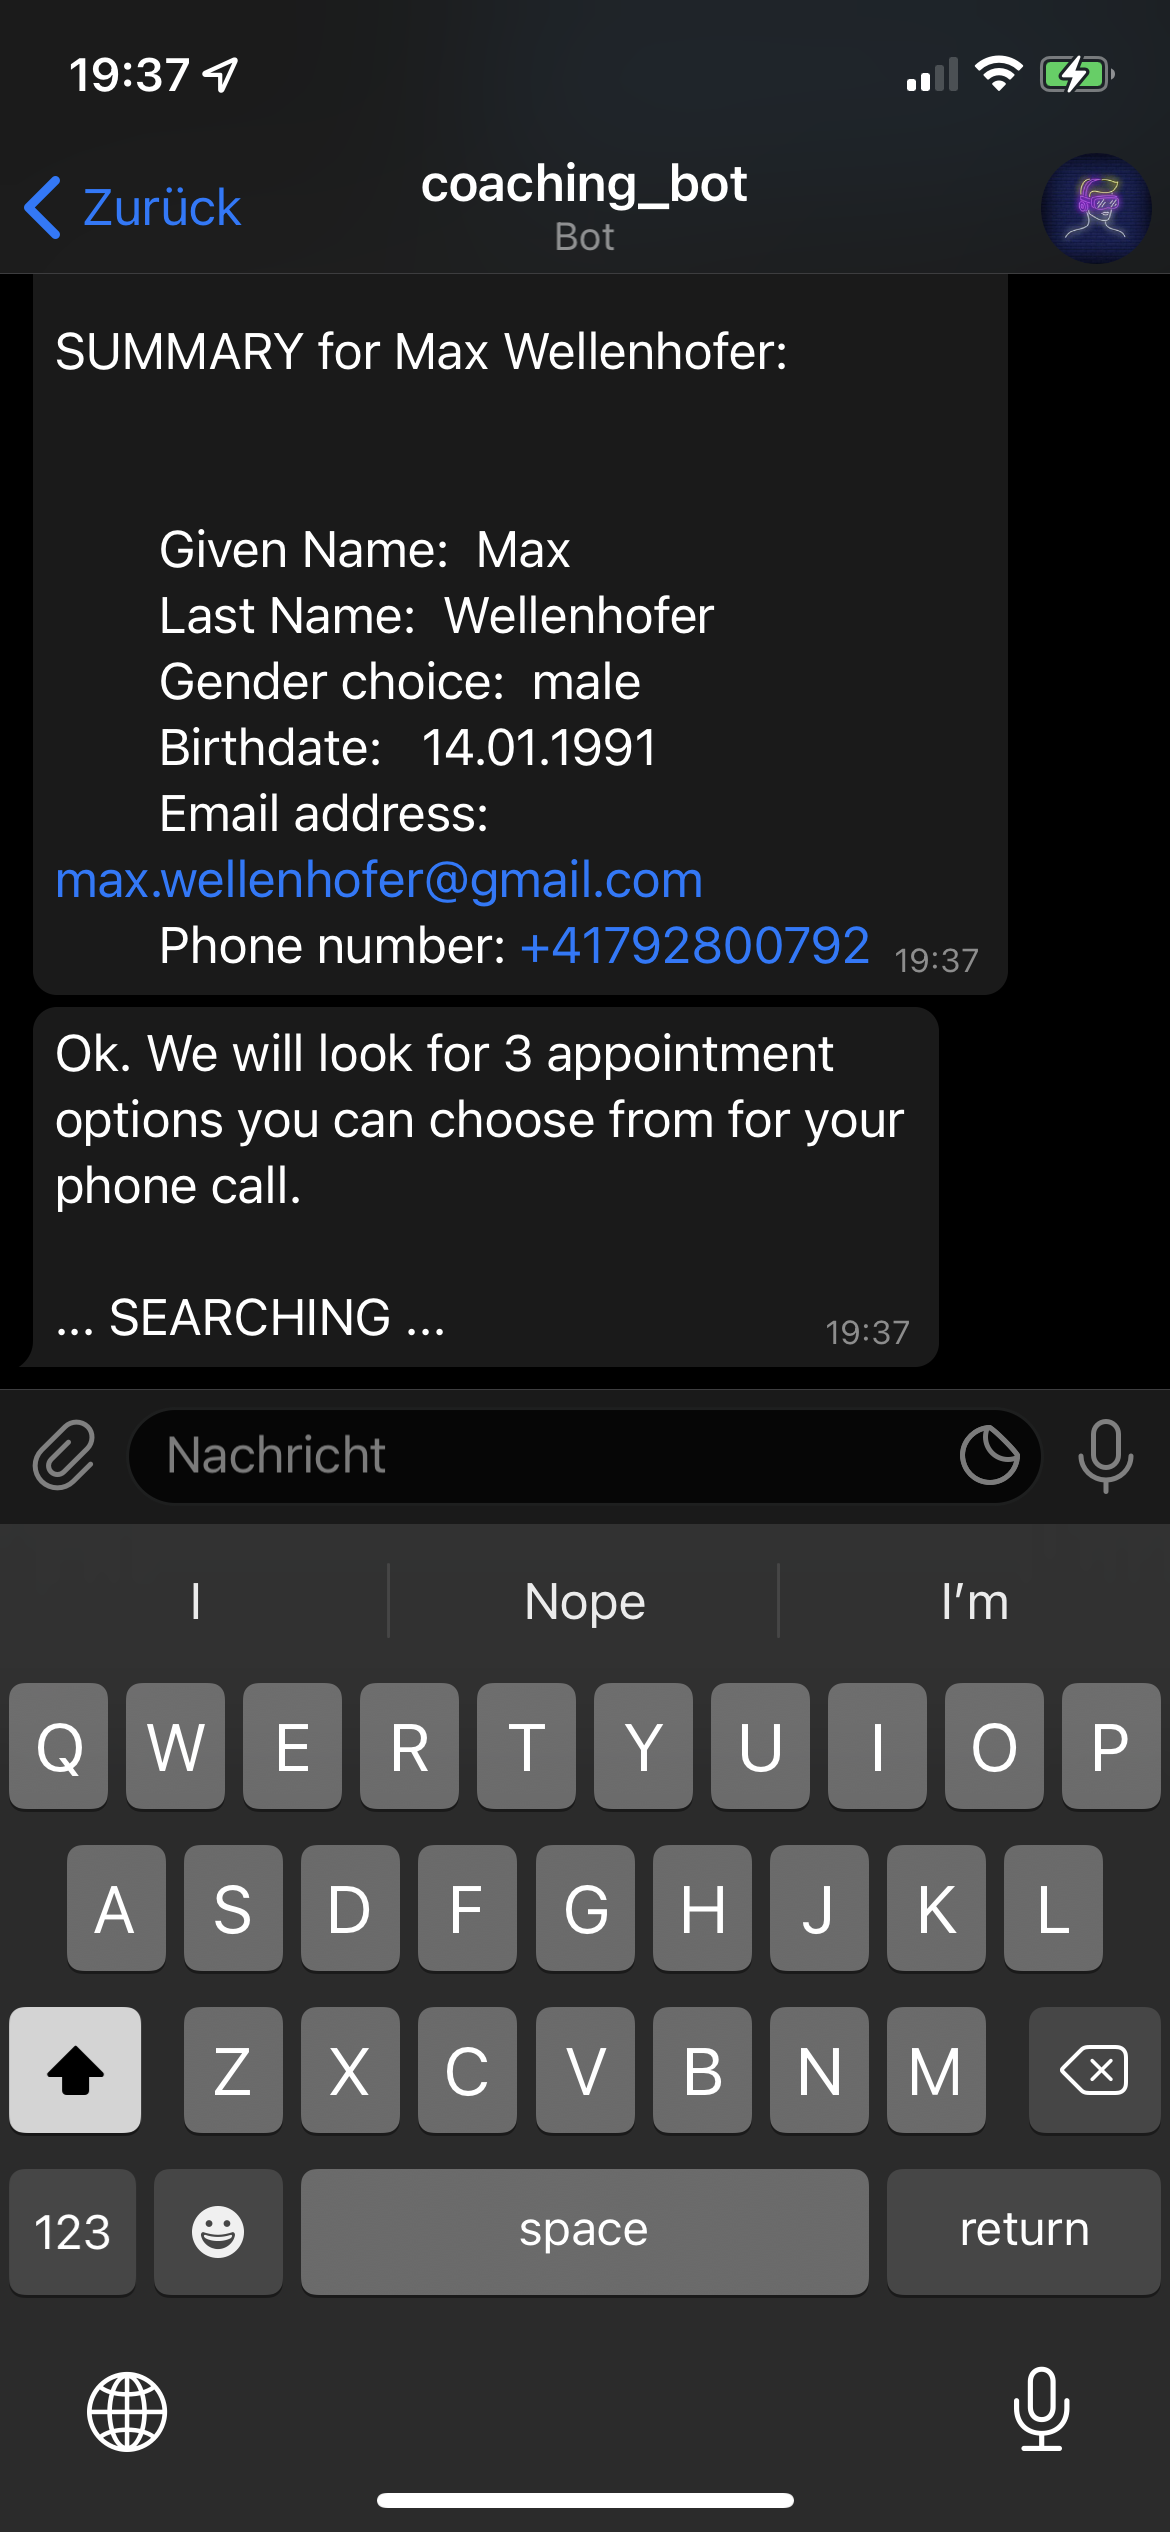
\includegraphics[width=0.4\textwidth]{images/Screenshots/slot-search.PNG}
		\caption{Terminfindung}
		\label{fig: scs..slot-search}
	\end{figure}


	\begin{figure}
		\centering
		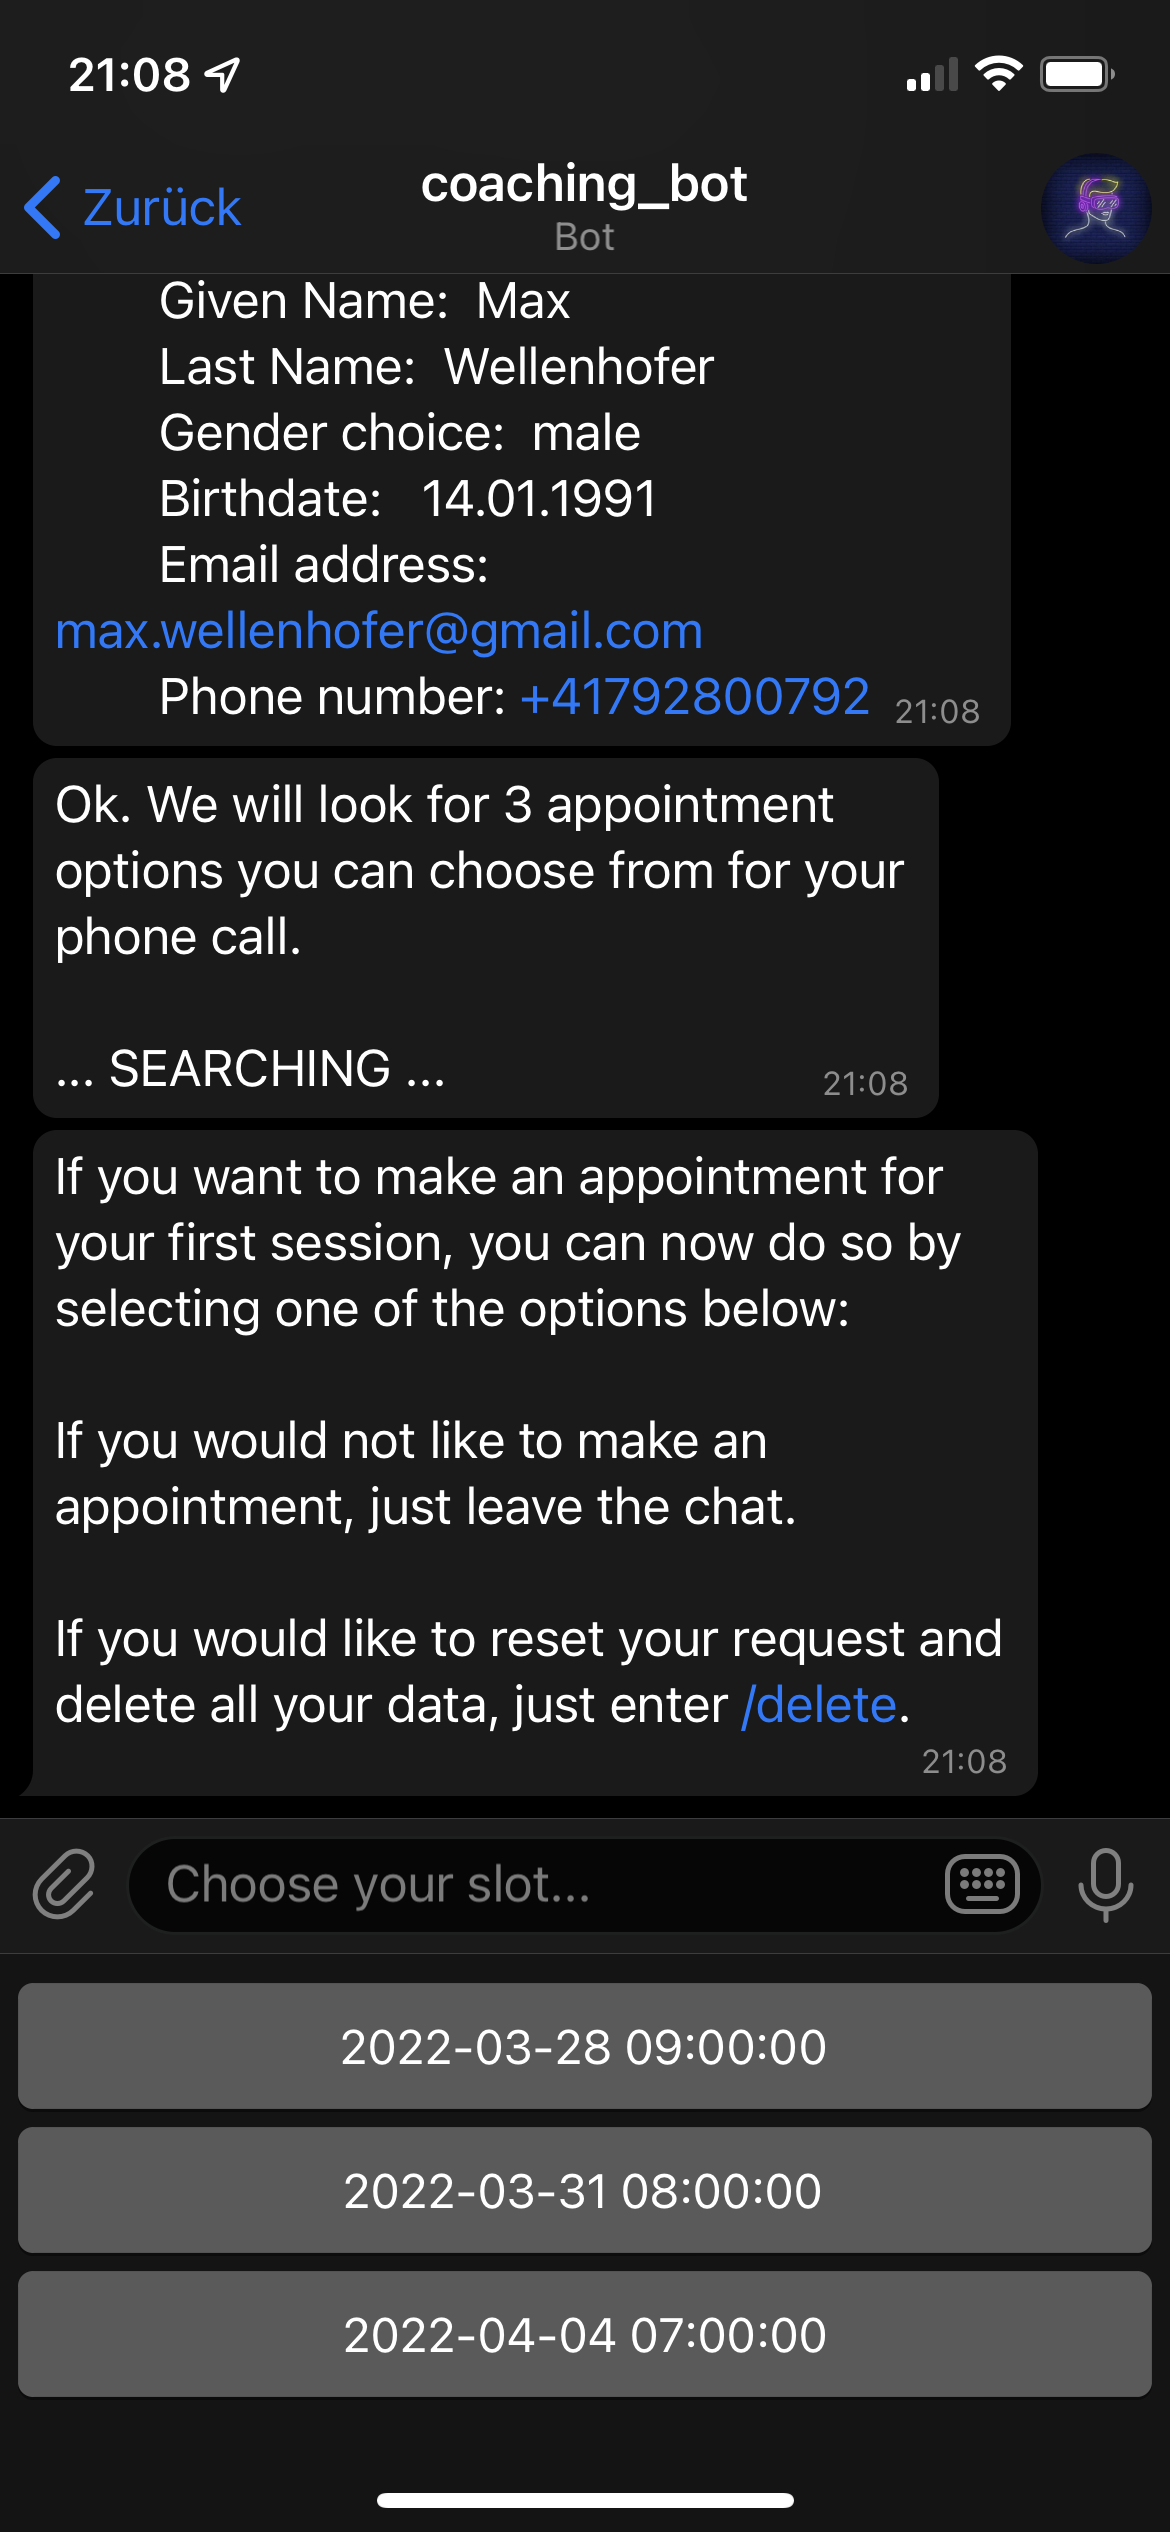
\includegraphics[width=0.4\textwidth]{images/Screenshots/appointment-selection.PNG}
		\caption{Terminauswahl}
		\label{fig: scs..appointment-selection}
	\end{figure}


	\begin{figure}
		\centering
		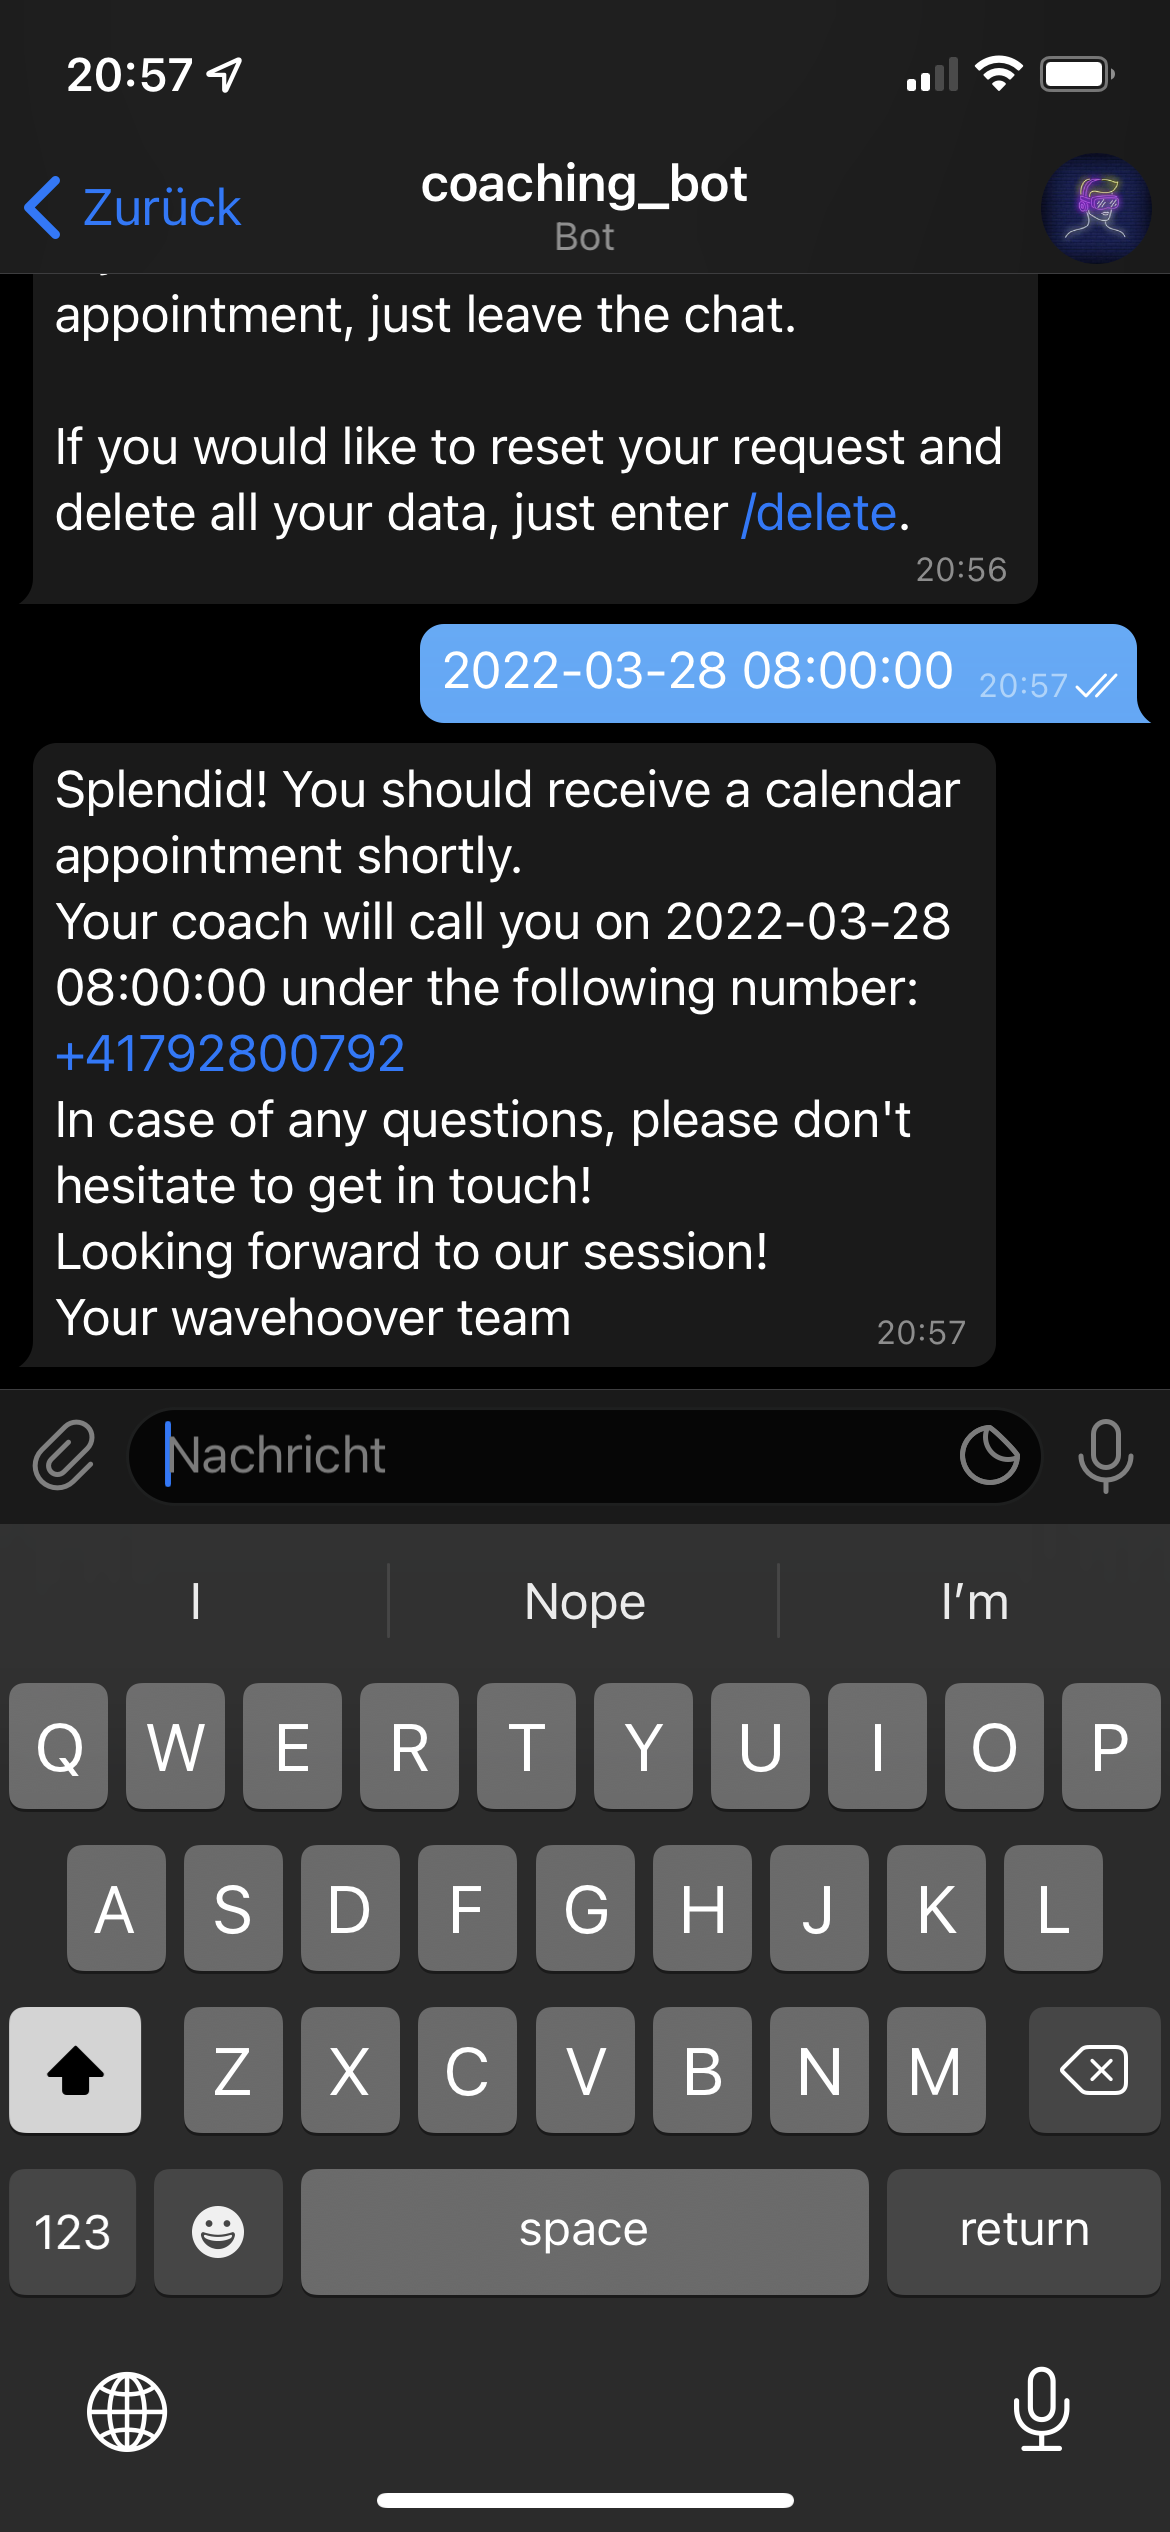
\includegraphics[width=0.4\textwidth]{images/Screenshots/appointment-made.PNG}
		\caption{Terminbestätigung}
		\label{fig: scs..Abbildung 10}
	\end{figure}


	\begin{figure}
		\centering
		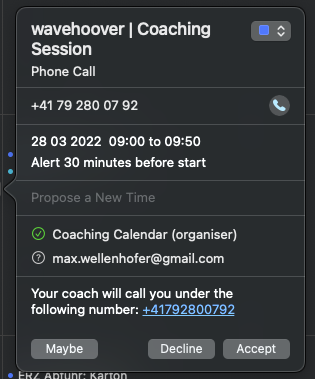
\includegraphics[width=0.4\textwidth]{images/Screenshots/calendar-invite.png}
		\caption{Kalendereinladung}
		\label{fig: scs..calendar-invite}
	\end{figure}


	\begin{figure}
		\centering
		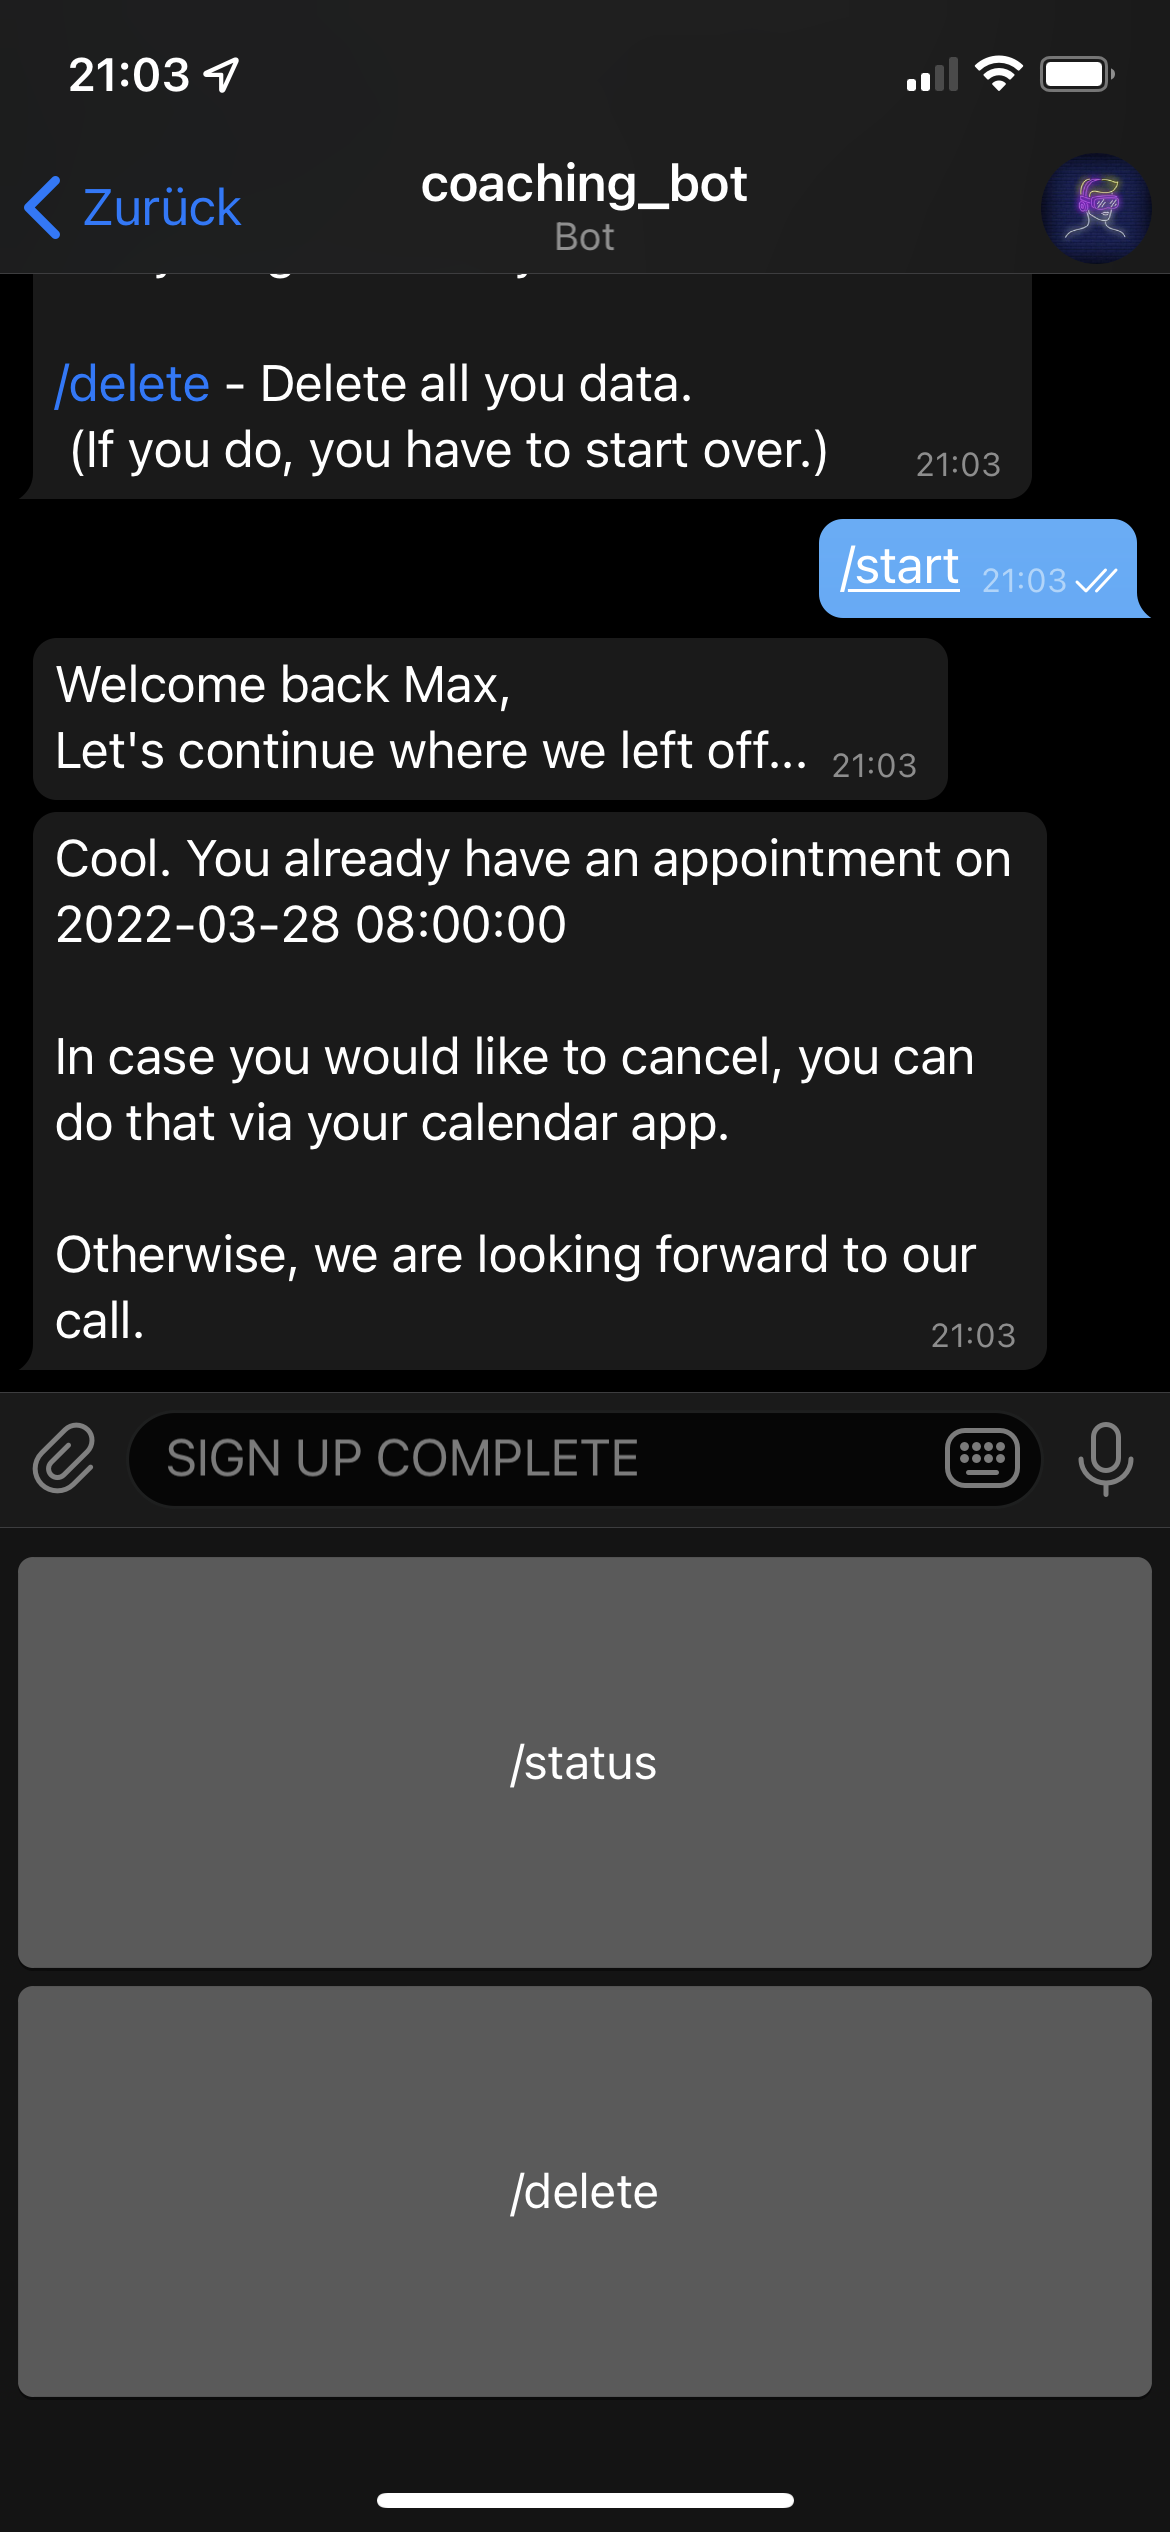
\includegraphics[width=0.4\textwidth]{images/Screenshots/return-with-appointment.PNG}
		\caption{Rückkehr zum Bot, wenn bereits ein Termin vereinbart wurde}
		\label{fig: scs..return-with-appointment}
	\end{figure}


	\begin{figure}
		\centering
		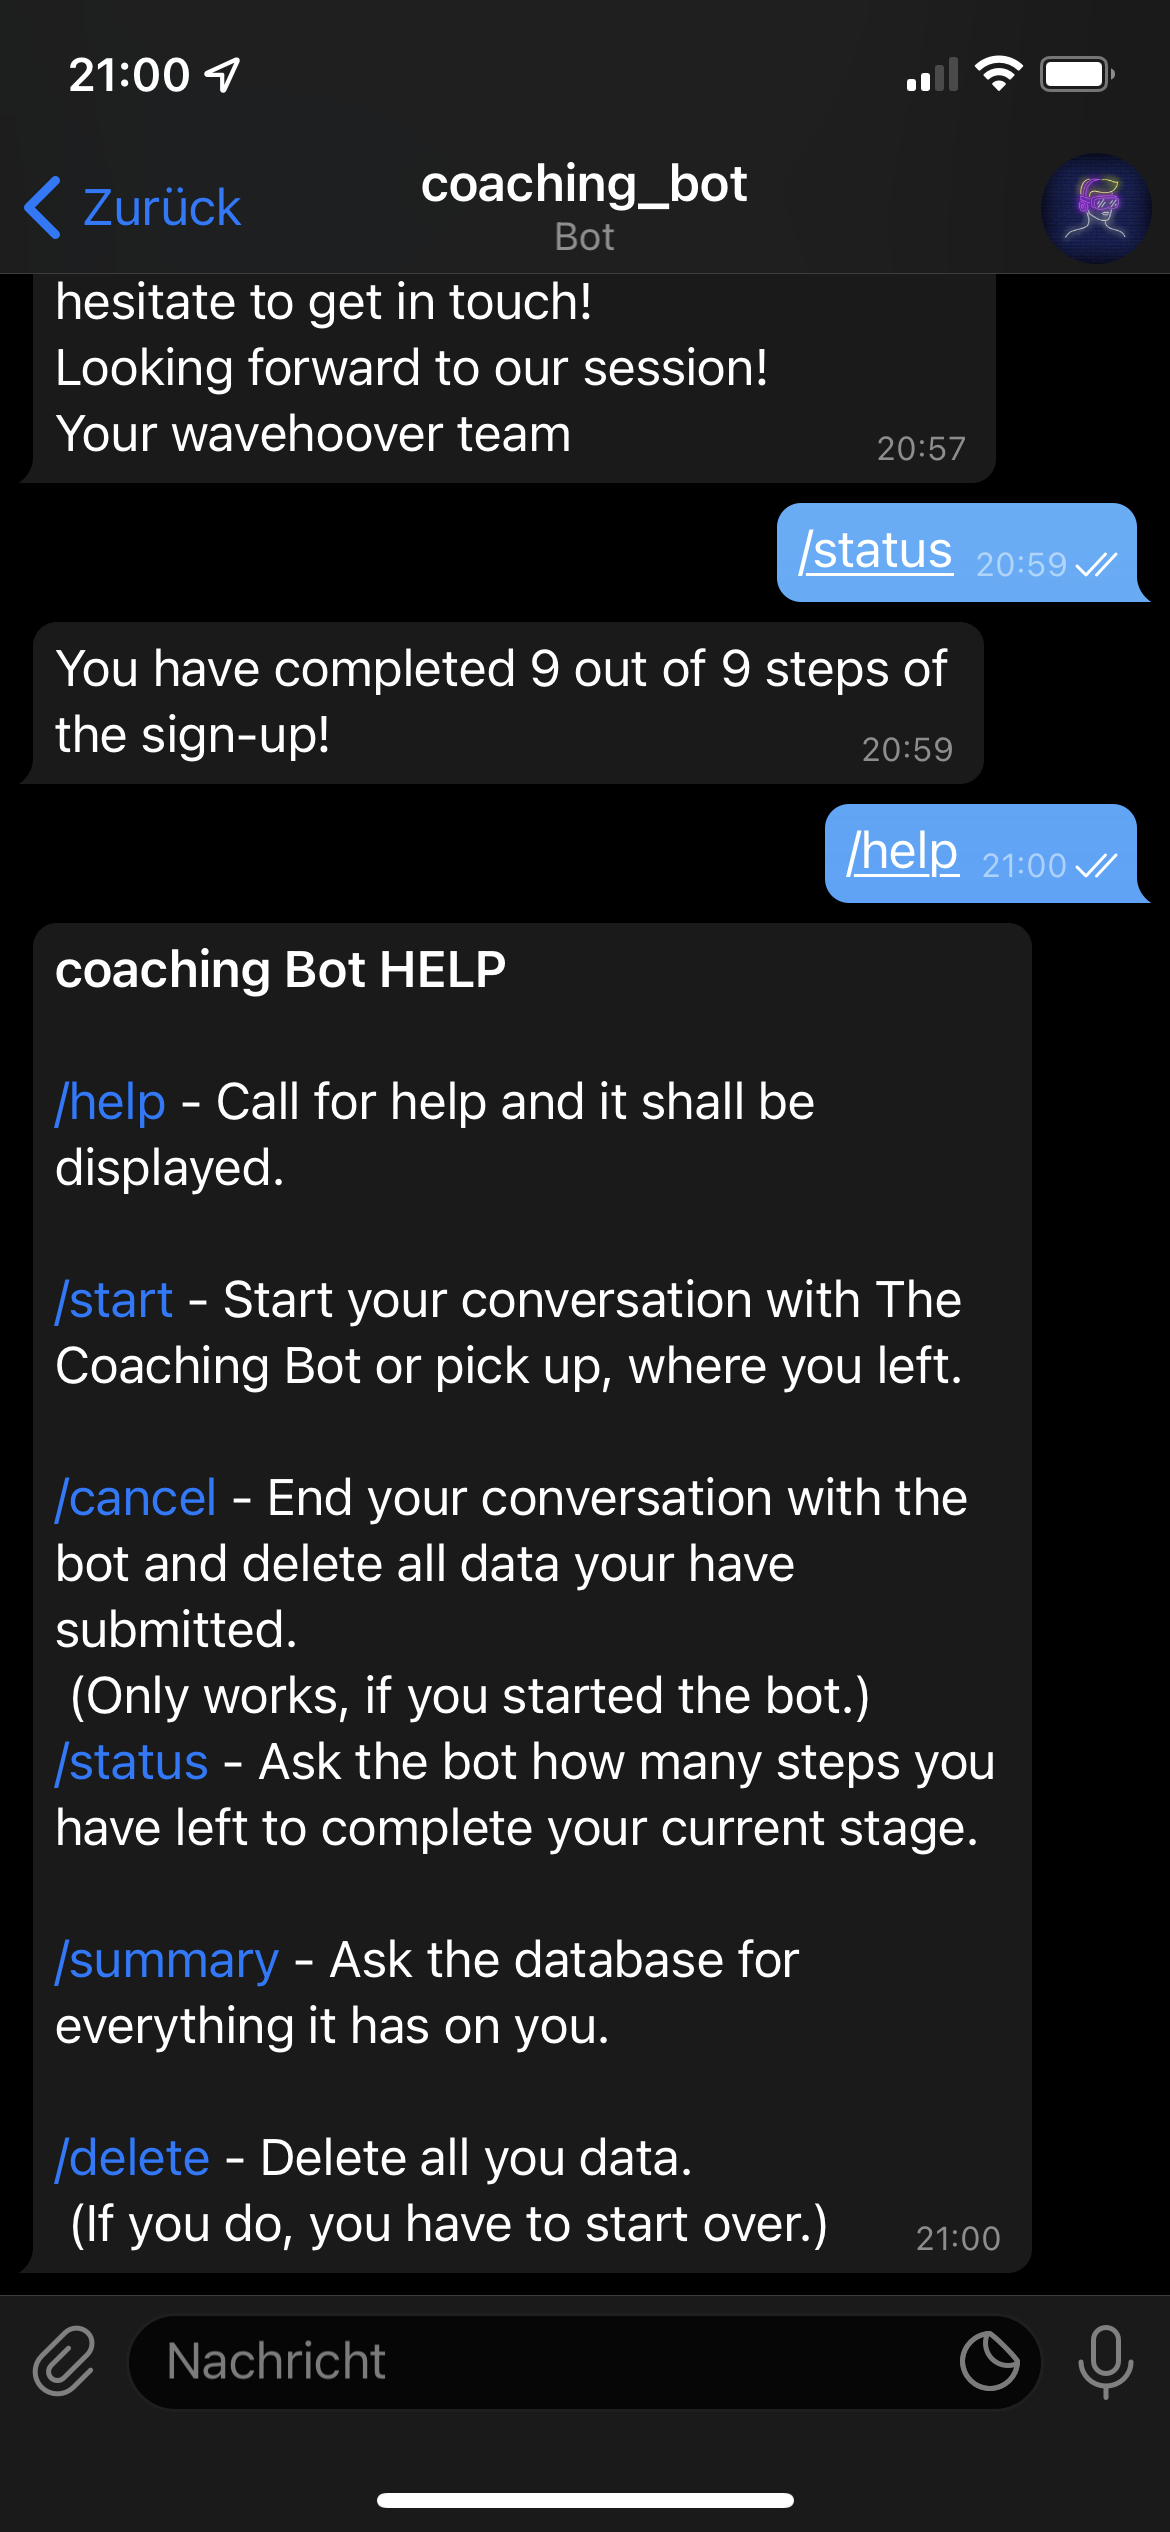
\includegraphics[width=0.4\textwidth]{images/Screenshots/status-and-help.PNG}
		\caption{Statusabfrage und Hilfe}
		\label{fig: scs..status-and-help}
	\end{figure}


	\begin{figure}
		\centering
		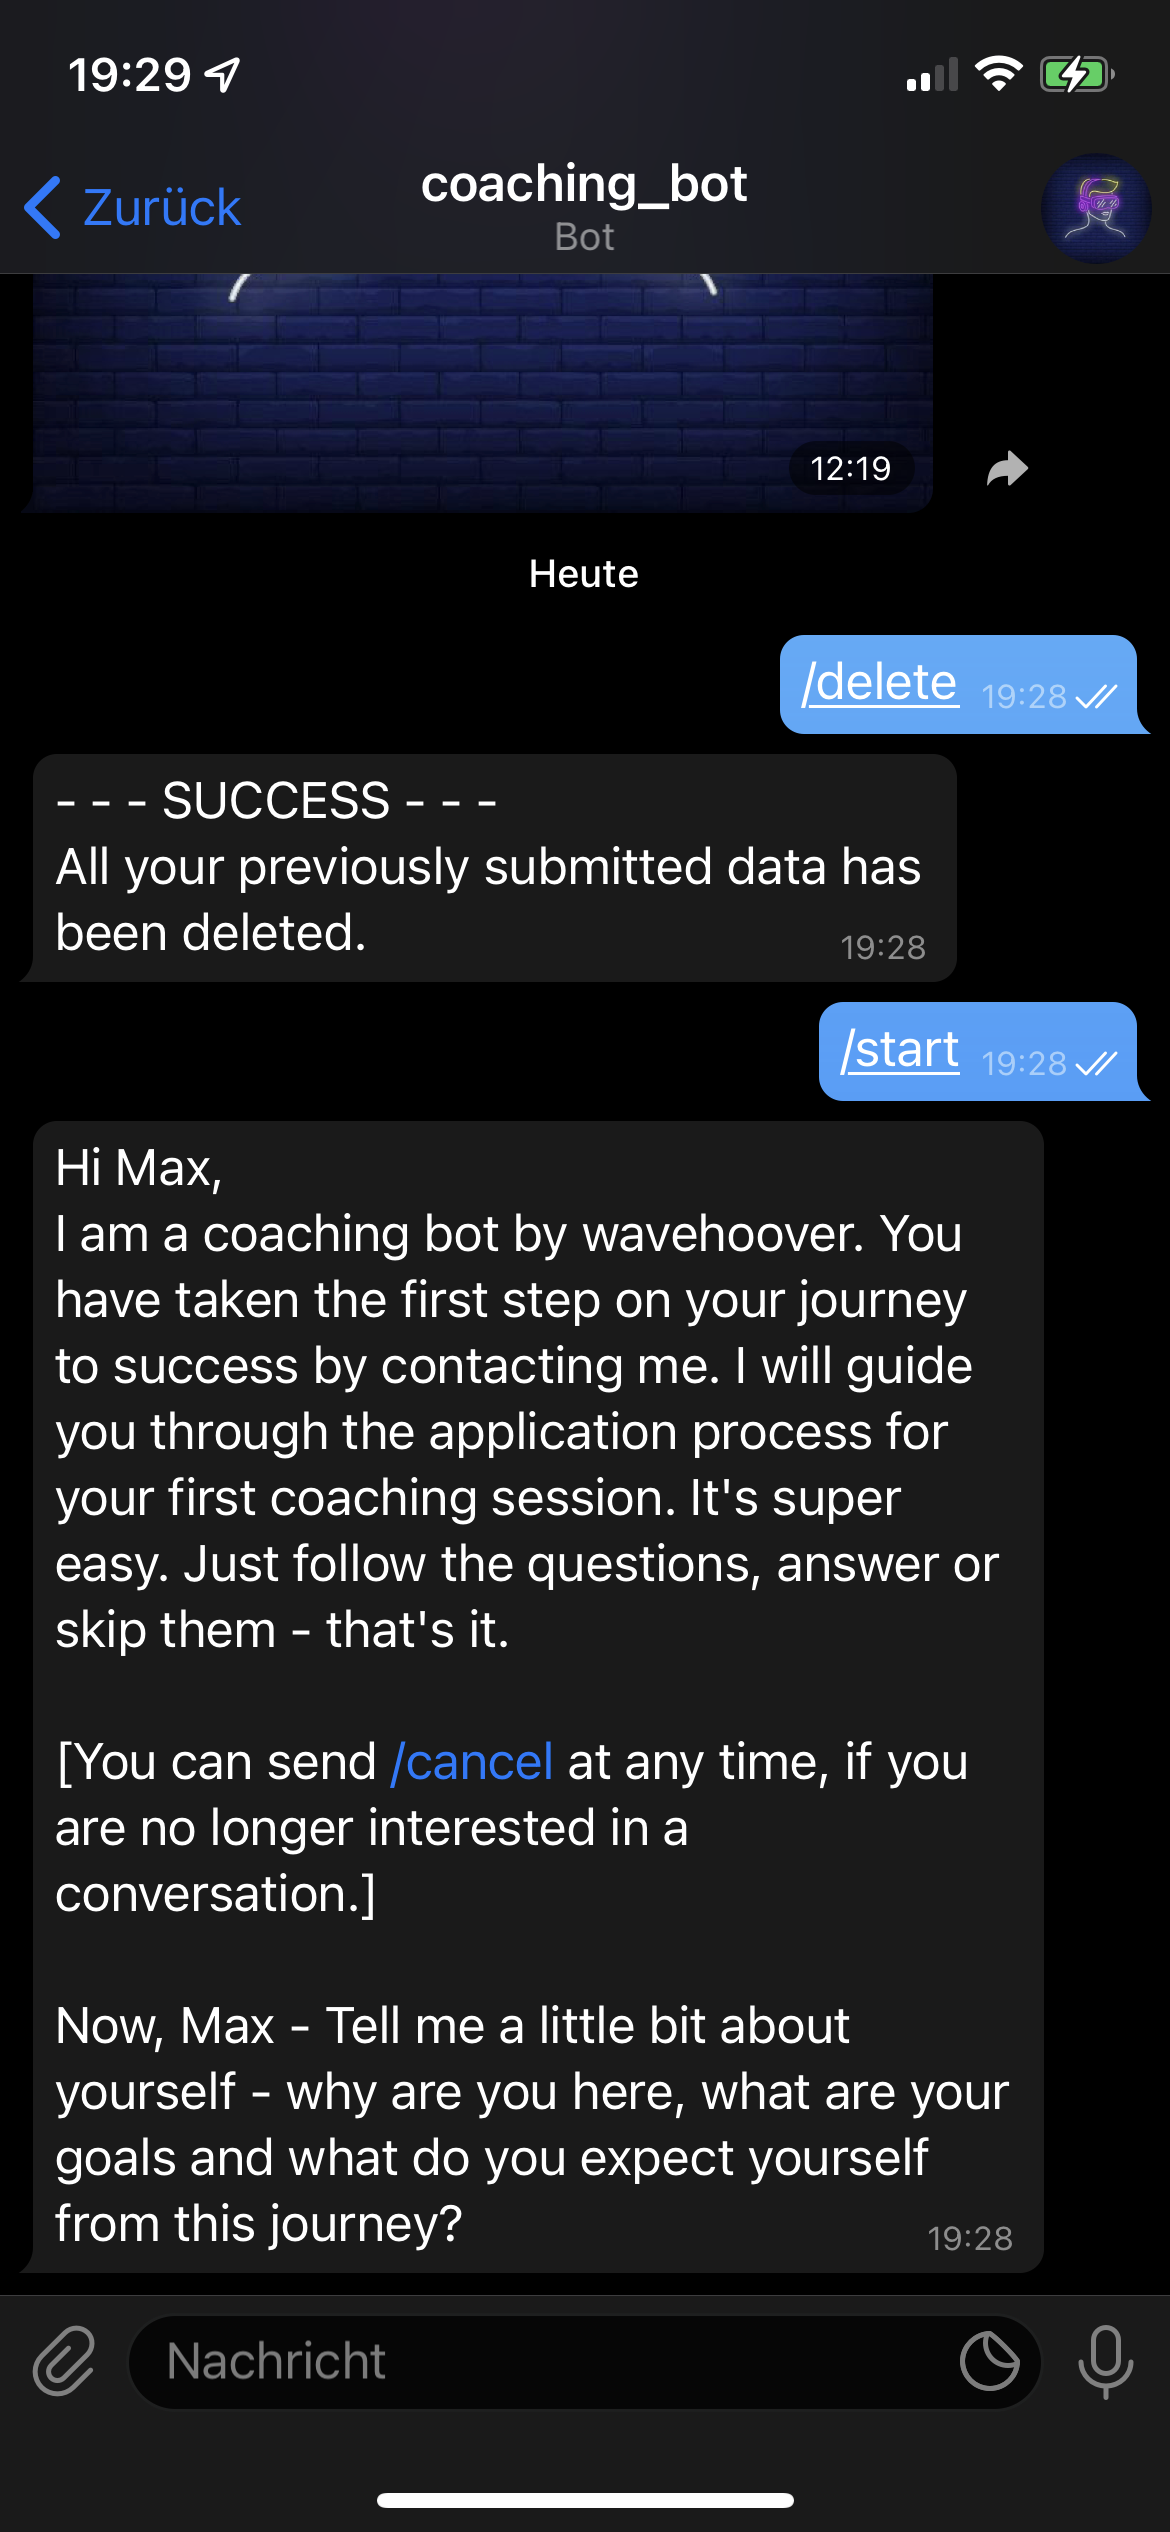
\includegraphics[width=0.4\textwidth]{images/Screenshots/delete-and-restart.PNG}
		\caption{Nutzerdaten löschen und Neustart des Bots}
		\label{fig: scs..delete-and-restart}
	\end{figure}


	\begin{figure}
		\centering
		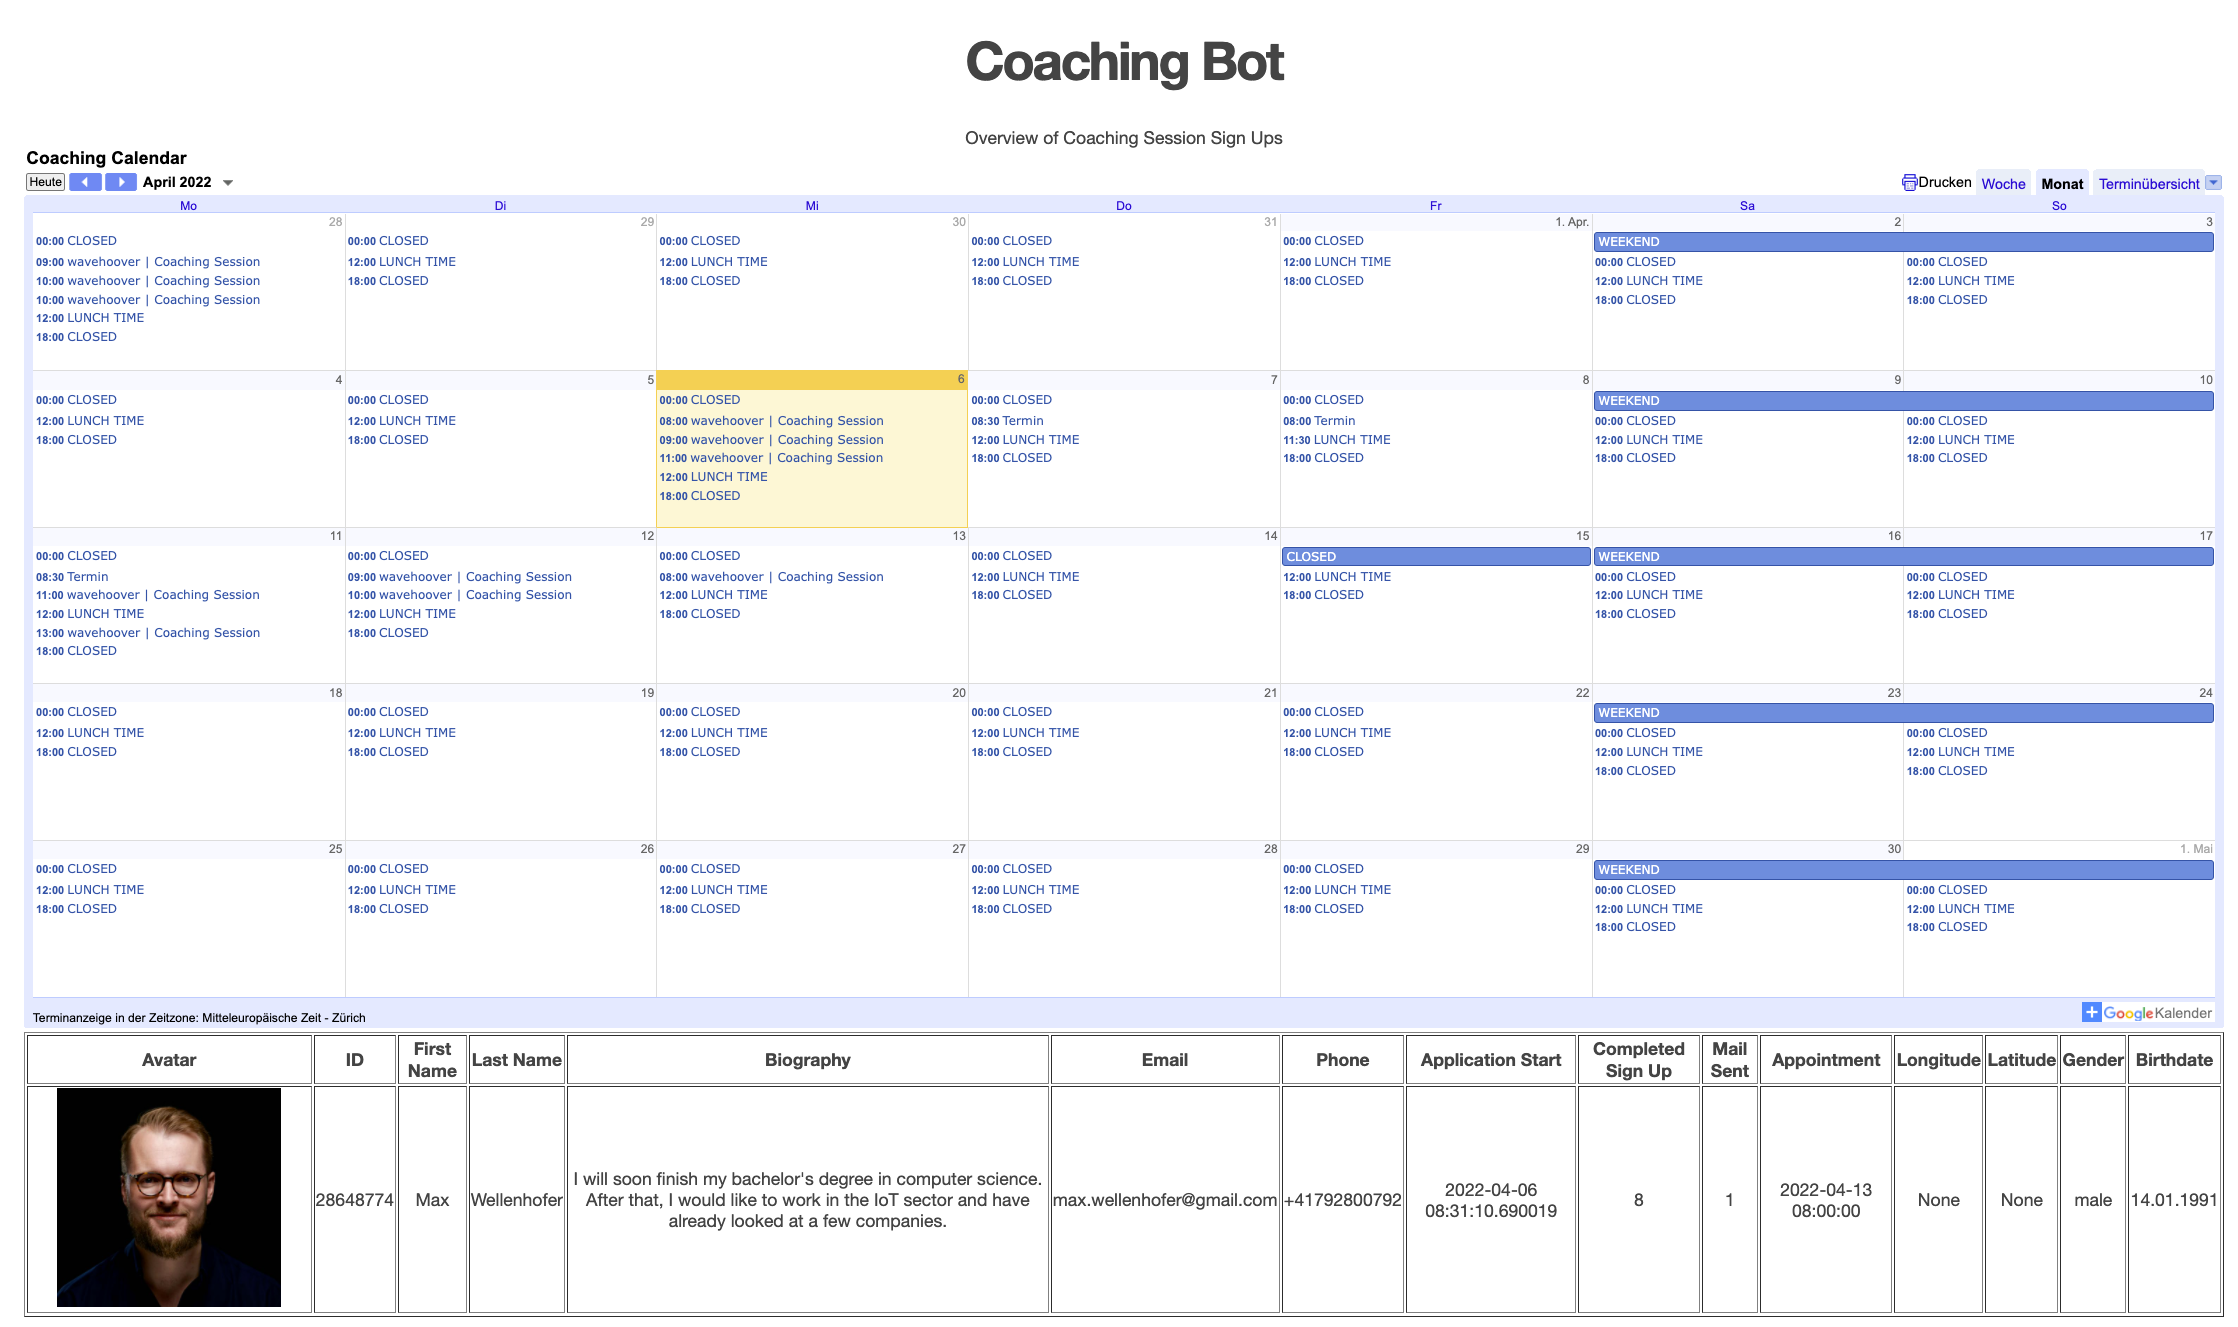
\includegraphics[width=0.4\textwidth]{images/Screenshots/web-gui.png}
		\caption{Ansicht Coach}
		\label{fig: scs..web-gui}
	\end{figure}

